\begin{savequote}[8cm]
    Once you've got a task to do, it's better to do it than live with the fear of it.
  \qauthor{--- Joe Abercrombie, \textit{The Blade Itself}}
\end{savequote}

\chapter{Topic modelling identifies novel PAF1c-bound enhancer elements in KMT2A-AFF1 leukemia patients}
\chaptermark{Topic modelling in fetal KMT2A-AFF1 Leukemia}
%\chapter{BLDA prioritizes accessible regulatory regions in MLL-AF4 driven leukemia} \label{ch4}

\minitoc


\section{Introduction} \label{ch5:intro}

% General statement of intent.
The \gls{mll} gene, previously known as MLL or MLL1, is a crucial epigenetic regulator required for definitive hematopoiesis \cite{Ernst2004a}. It is also frequently involved in chromosomal translocations causing a treatment resistant leukemia with especially poor prognosis \cite{Krivtsov2007}. Though outcomes for acute leukemias in children has improved vastly, the five year event-free survival rate for infant leukemias remains less than 50\% despite extensive treatment efforts and supportive care \cite{Rice2020}. Recent work has demonstrated the important roles of chromatin remodelling in KMT2A-recombinant (KMT2Ar) leukemiagenesis, though the specifics of the differentially accessible regulatory programs active in infant KMT2Ar remains unknown \cite{Erfurth2003}. In this chapter, I propose the use of the previously developed topic modelling approach BLDA to identify accessible regulatory programs in KMT2A-AFF1 leukemia patients.  

KMT2A is expressed ubiquitously throughout haematopoiesis, playing an crucial role in maintaining normal numbers of progenitor cells and ensuring the availability of adult \glspl{hsc} \cite{Meyer2017, Antunes2020, Ernst2004} . Its deletion is embryonically lethal in mice, illuminating its role in stage specific control of gene expression. Much of the original work of characterizing its function as a transcriptional regulator came from model systems due to a close homology to Trithroax in \textit{Drosophila} and similar activity to SET1 (aka COMPASS) in yeast \cite{Popovic2005}. Similar to the yeast analog SET1, a C-terminal SET domain confers histone H3K4 methyltransferase activity while the N-terminal is responsible for binding with three AT-hook motifs and four PHD fingers \cite{JJ2003, Hsieh2003}. While functional, KMT2A is responsible for region specific methylation deposition responsible for a diverse set of functions including marking enhancer elements and promoting transcription initiation \cite{Wang2009}. In KMT2Ar driven leukemias, the cleaved N terminus instead associates with one of up to ninety C-terminal proteins, conferring a huge range of functional activities and interupting its normal function as a methyltransferase \cite{Hsieh2003}. The fusion (KMT2A-FP) is able to recruit new cofactors such as DOT1L, whose abberant methylation profile at H3K79 sites is highly discriminatory for genes activated by the fusion protein and believed to be crucial for the transforming activity of KMT2A-FPs \cite{YOkada2005, KMBernt2011}. Incidentally, clinically targeting DOT1L is generally not sufficient to have any effect on many KMT2Ar cell lines, though some early evidence suggests that targetting DOT1L alongside other key cofactors like menin may show more success \cite{Dafflon2016}. This demonstrates the resiliency and redundancy in KMT2A-FP driven leukemias, and the need to understand the full complement of epigenomic changes involved in leukemia maintenance.  

Much like its analog COMPASS, KMT2A has an intimate relationship with chromatin remodelling factors such as INI1 and SNF5 \cite{Cenik2021, Sugeedha2021}. This family of epigenetic modifiers termed SWI/SNF (historically called SWItch/Sucrose non-fermentable due to its involvement in yeast sucrose fermentation pathways) was first characterized in yeast, and is involved in ATP-dependant nucleosome mobilization during transcription and the cell cycle \cite{C2015}. In humans, mutations within SWI/SNF chromatin remodelling complexes are incredibly common in cancer; as an example, 57\% of ovarian clear cell carcinomas contained inactivating mutations along the length of a BAF complex subunit ARID1A (ref 45). Similarly, inactivation of INI1 causes a rare and extremely aggressive childhood cancer called malignant rhabdoid tumours (MRTs), nominating INI1 as a recessive tumor suppressor and raising key questions about its dysregulation in KMT2Ar cancers due to direct protein-protein interactions \cite{I1998}. See \cite{C2015} for a comprehensive review of the roles of the human SWI/SNF complex in malignancies. 

% Alongside COMPASS, this family of proteins competes with PgC proteins to activate important genes such as HOXA9 during development, and human analogs  

% Paragraph about the disease itself. 
Translocations involving KMT2A are a negative pronostic factor when the leukemia presents as \gls{all}, but not as \gls{aml} in infants \cite{Meyer2014}. The former, however, accounts for upwards of 80\% of leukemias involving KMT2Ar \cite{Rice2020}. The reasons for this difference in prognosis are not well understood, especially as cancers with this etiology are especially plastic with regards to their presentation. Leukemias initially presenting as \gls{all} often present as \glspl{aml} upon relapse (which is a frequent occurance among KNT2Ar leukemias).  however the underlying chromatin landscape of the cancer cells in this case is able to produce gene expression programs resembling either of the two diseases, or a phenotypically intermediate form known as mixed lineage leukemia (MLL). Though KMT2A has well described direct interactions with many different proteins including cell cycle regulators like E2F and HCF, Cyp33, HDAC complexes, histone acetylases (CBP and P300) and the previously mentioned chromatin remodelling factors INI1 and SNF5, the degree to which the fusion proteins influence the transcriptome is only just beginning to be illuminated \cite{Sugeedha2021}. Its affinity for binding to specific regions of the genome is not entirely determined by the actual sequence but also partially the structure of the DNA, with early results indicating binding affinity for cruciform DNAs with no clear sequence homology \cite{NJ1994}. Much recent research points to disturbances in the epigenetic regulation of gene expression as a potential mechanism for leukemiagenesis \cite{Krivtsov2007}.

In this chapter, I concentrate on the most frequent fusion partner of KMT2A, AFF1 or AF4 as it was previously known \cite{Meyer2017}. Many fusion partners of KMT2A belong to a network of transcriptional regulators involved in chromatin remodeling, including AF4, and the disruption of this network may be important for leuekmiagenesis \cite{Erfurth2003}. In fact, recent evidence has suggested that the KMT2A-AFF1 fusion protein is involved in a complex feed-forward gene regulatory network (GRN) involving many well-known proteins such as RUNX1 and CASP9 as well as some which have no previously-described function \cite{Harman2021, Wilkinson2013}. Outside of well-characterised direct binding events where KMT2A-AFF1 is able to regulate the expression of key genes such as proto-oncogene MyC and BCL2, its regulation of and interactions with downstream gene targets is almost completely unknown. This is especially true in the case of infant leukemias with dismal prognosis, where a unique fetal-specific gene expression profile may contribute to the otherwise unexplained age-related differences in prognosis \cite{Rice2020a}. Fetal lymphopoiesis remains poorly defined, however clearly defining the expression and accessibility profiles as they differ from adult progenitor cells is key to understanding leukemiagenesis. Recently, two CD19$^+$ B-cell progenitors were identified in fetal populations, a CD10$^+$ ProB (PB) cell type resembling adult progenitors and a completely novel Pre-ProB (PPB) CD10$^-$ celltype almost undetectable in adult bone marrow \cite{OByrne2019}. Additionally, their transcriptomic profile is dissimilar from the small numbers of PPB cells able to isolated in adults, and share expression signatures with CD10$^-$ infant \gls{all} blast cells \cite{OByrne2019}. These cells therefore represent the earliest identified fetal-restricted committed lymphoid progenitor, suggesting that they may provide a permissive environment for leukemia origination.  

This chapter aims to use topic modelling to describe regulatory programs within four childhood leukemia patients, contrasting them against two closely related healthy fetal cell types, PB, and PPB. We also compare these samples against two cellular models of KMT2A-AFF1, RS411 and SEM, both derived from childhood leukemias. I use the previously developed BLDA method to identify key-word regions discriminative of the different groupings of samples, and study their epigenomic properties. This amounts to an investigation into the accessible regulatory regions and pathways active in in this uniquely difficult to treat form of leukemia. 

% Some leukemias are maintained by populations of self-renewing \glspl{lsc}, possibly originating from early stage \glspl{hsc}. However, one binding partner for KMT2A, ENL, has shown to be able to create populations of LSCs from later stage, lineage committed myeloid progenitor cells. This  


% Beyond menin, KMT2A has been shown to interact with 



% About MLL
% - Found in upwards of 70\% of infant leukemias (AML + ALL)
% - Decreased in older children. Also found in treatment induced leukemias. 10\% overall leukemias. 
% - MLL-r ALL + leukemias after topoisomerase II inhibitors have bad outomes. Weirdly, AML with MLL-r has same prognosis. d
% - Some leukemias are maintained by populations of self-renewing LSCs, HSCs could be the cell of origin for chronic and acute myeloid leukaemias. This is because they are long lived and capable of proliferation. 
%     - Reya, T., Morrison, S. J., Clarke, M. F. & Weissman, I. L. Stem cells, cancer, and cancer stem cells. Nature 414, 105–111 (2001).
% - However, some experiments show that committedd myeloid cells can be transformed to LSCs if they express MLL-ENL (though it required a larger number)

% - MLL is ubiquitously expressed throughout hematopoiesis. SET domain that is responsible for methylation of H3K4 similar to SET1 in yeast. AF4 is also known as AFF1



% - HoxA9 is important. Menin is required to supress MLL from messing up HOXA9 expression, important for transformation 
%     - Yokoyama, A. et al. The menin tumor suppressor protein is an essential oncogenic cofactor for MLL-associated leukemogenesis. Cell 123, 207–218 (2005).
% - Positively influenced gene expression for some things like HOX genes
% - HOX genes expression is initiated properly but not maintaind will MLL fusions 
%     - Yu, B. D., Hess, J. L., Horning, S. E., Brown, G. A. & Korsmeyer, S. J. Altered Hox expression and segmental identity in Mll-mutant mice. Nature 378, 505–508 (1995).

% - Disturbance in the epigenetic regulation of gene expression as a potential mechanism for human leukaemogenesis. 
% - AF4 is the most common and the one that we will concentrating our study on
% - AF4 has C terminal transriptional activation.
% - Many MLL fusion partners belong to a network involved in transcriptional regulation through chromatin remodelling 
%     - Erfurth, F., Hemenway, C. S., de Erkenez, A. C. & Domer, P. H. MLL fusion partners AF4 and AF9 interact at subnuclear foci. Leukemia 18, 92–102 (2004).
% - E.x. AF10 associated with DOT1L, DOT1L is important for MLL-AF10 activity. If DOT1L was inactivated, either through small interfering RNAs or by using a catalytically ianctive mutant, MLL-AF10 was unable to transform haematopoietic progenitors into leukemia stem cells
%     - Okada, Y. et al. hDOT1L links histone methylation to leukemogenesis. Cell 121, 167–178 (2005). Identifies a unique function of an MLL fusion (MLL–AF10). The recruitment of the H3K79 methyltransferase DOT1L by AF10 is necessary for transformation.
% - MLL-ENL, H3K79me increased on HOXA9 and MEIS1 promoters 
%     - Milne, T. A., Martin, M. E., Brock, H. W., Slany, R. K. & Hess, J. L. Leukemogenic MLL fusion proteins bind across a broad region of the Hox a9 locus, promoting transcription and multiple histone modifications. Cancer Res. 65, 11367–11374 (2005).


% - Not reaaaaaaly sequence specific 
%     - Zeleznik-Le, N. J., Harden, A. M. & Rowley, J. D. 11q23 translocations split the “AT-hook” cruciform DNA-binding region and the transcriptional repression domain from the activation domain of the mixed-lineage leukemia (MLL) gene. Proc. Natl Acad. Sci. USA 91, 10610–10614 (1994).
% - Of all the binding partners, AF4 (t(4;11)(q21;q23)) is the most common, AF4 belongs to an expanding family of serine / proline rich nuclear proteins. 
%     - Meyer C, Hofmann J, Burmeister T, Gröger D, Park TS, Emerenciano M, Pombo de Oliveira M,
%     Renneville A, Villarese P, Macintyre E, et al. 2013. The MLL recombinome of acute leukemias
%     in 2013. Leukemia 27: 2165–2176. 
% - KMT2A-FP is able to drive leukemogenesis alone through aberrant gene expression profiles. 
% - KMT2A-AFF1 most often resembles ALL, but can also look like either AML or a mixed phenotype leukemia. They can also relapse to become AMLs derived from a clone of the original leukemia. This indicates a core network of genes differentially regulated in KMT2A-AFF1 leukemia that can drive both AML and ALL.
% - Though key genes are important, a lot of key regulation is caused by entire networks of genes 
%     - Reik W. 2007. Stability and flexibility of epigenetic gene regulation in mammalian development.
%     Nature 447: 425–432. 
% - Though it is worth mentioning that some genes are just disease induced, and not all differentially expressed genes are actually involved in the disease
%     - https://www.nature.com/articles/s41467-021-25805-y
% - Direct binding is implicated in key genes like BCL2 and proto-oncogene MYC as well as RUNX1 
%     - Guenther MG, Lawton LN, Rozovskaia T, Frampton GM, Levine SS, Volkert TL, Croce CM, Nakamura
%     T, Canaani E, Young RA. 2008. Aberrant chromatin at genes encoding stem cell regulators in
%     human mixed-lineage leukemia. Genes Dev 22: 3403–3408. 
%         - This one looks important regardless 
% - Direct binding events show grossly different profiles of chromatin structure, histone modifications very different. 

% - Direct binding is not all that is important. GRN showed that RUNX1 is very important. Also represesses CASP9. 
%     - Joe's paper
% - Very few cooperating mutations
%     -Bardini M, Galbiati M, Lettieri A, Bungaro S, Gorletta TA, Biondi A, Cazzaniga G. 2011.
%     Implementation of array based whole-genome high-resolution technologies confirms the
%     absence of secondary copy-number alterations in MLL-AF4-positive infant ALL patients.
%     Leukemia 25: 175–178.  



\section{Results} \label{ch5:results}



\subsection{Data Processing and Peak Calling}

We perform \gls{atac} on four childhood leukemia patient samples from the \gls{ukbb} as well as two cellular models of KMT2A-AFF1 leukemia, RS411 and SEM. Details of the processing of these samples and the maintenance of cell lines is available in the Methods section. We collect three Pre-ProB (PPB) and three ProB samples from previous work and download coverage data from the Gene Expression Omnibus (GEO) \cite{OByrne2019}.  

% Within the context of the entire ENCODE dataset, the MLL-AF4 cells were indistinguishable from the closely related B cell precursors. In order to identify differences between them, the model would need a very large number of topics, sufficient to explain all of the detailed similarities between the diverse set of celltypes represented in the dataset. This is computationally difficult, and risks over-parameterizing the data. A reasonable alternative is a detailed examination of these cells in isolation, and a comparison to the results generated in the larger model. In this section, I create a topic model with just the cells of interest and attempt to differentiate them based on patterns in accessible chromatin using BLDA.

We use lanceotron to define peaks representing accessible sequence from the different samples. The number of called peaks differed significantly between experiments (\Cref{fig:mll_peak_calls}A). The most peaks were found in SEM and RS4;11, and the fewest were identified in Patient 3. In the latter case, it is suspected that the known low quality of this sample affected the sequencing, causing an anomalously low number of peaks to be identified. To confirm this, we use megadepth to calculate the average read coverage under identified peak regions \cite{Wilks2021} (\Cref{table:mll_cov}). Unexpectedly, patient 2 showed comparable read coverage to the other samples, while Patient 3 had anomalously low read coverage under the identified peak regions. An unremarkable number of peaks were identified in patient 3. The remainder of the samples have high coverage values sufficient to identify high quality peaks. These results encourage caution when interpreting any topic modelling on both patients 2 and 3.  


% Please add the following required packages to your document preamble:
% \usepackage{booktabs}
\begin{table}[]
    \centering
    \begin{tabular}{@{}llr@{}}
    \toprule
    Sample Identifier & Sample Alias & Coverage \\ \midrule
    Patient 11911     & Patient 1    & 884.3                        \\
    Patient 21940     & Patient 2    & 801.0                        \\
    Patient 26754     & Patient 3    & 478.8                        \\
    Patient 27800     & Patient 4    & 809.2                        \\
    PPB\_95R          & PPB 1        & 1361.5                       \\
    PPB\_75           & PPB 2        & 1610.6                       \\
    PPB\_23           & PPB 3        & 1295.9                       \\
    PB\_95R           & PB 1         & 1776.3                       \\
    PB\_75            & PB 2         & 1242.6                       \\
    PB\_23            & PB 3         & 1405.6                       \\
    RS411             & RS411        & 701.8                        \\
    SEM               & SEM          & 725.3                        \\ \bottomrule
    \end{tabular}
    \caption{Average coverage in peak regions for each sample calculated with megadepth.}
    \label{table:mll_cov}
\end{table}

Here we are comparing two methods, BLDA and cisTopic. cisTopic uses as its input a binary accessibility matrix, while BLDA uses a quantitative measure of relative coverage. To understand the structure of input to cisTopic, we plot the number of shared peak regions between the samples (\Cref{fig:mll_peak_calls}). Patient samples are overall dissimilar from \gls{bcp} and the cell lines. Consistent with the number of available peak calls, patient 2 shares the fewest peaks with the other samples. This is explainable by the low numbers of peaks in patient 2 in general. Between the two cell lines, SEM shares significantly more peaks with the \gls{bcp} than RS4;11 does (paired $T$-test P=2.56e-4). Surprisingly, there is no evidence for increased sharing within either PPB or PB cells ($T$-test P=0.595). These patterns of sharing will be important when interpreting the raw differential peak topic modelling versus the qualitative BLDA results.

\subsection{An MLL-AF4 specific accessibility blacklist} \label{mll_blacklist}

Cell lines maintained in culture accumulate genetic differences over time, some of which may be advantageous to their survival in culture. \cite{Liu2019}\textcite{Ben-David2018} studied the genetic baseline for the same cell line matured in different laboratories and identified copy number gains and loses, insertions and deletions (indels) and chromosomal translocations affecting large portions of the genome in cell lines which were not shared across laboratories. Latent structural differences between the cell lines in question and the reference genome pose a particularly concerning confounding factor to the interpretation of topic modelling; differences in mappability between regions reflected in abnormal peaks unrelated to biological differences between cell types would contaminate pathway and motif enrichment analyses. To ameliorate concerns associated with structural diversity in the RS4;11 and SEM cell lines within our laboratory environment, we construct a list of regions whose enrichment is solely due to technical issues such as biases in mappability.

% These numbers are still fine
To do so, we assemble collection of input tracks to ChIP-seq analysis conducted on the RS4;11 and SEM cells in question. Briefly, these input tracks represent sonicated DNA that has not been pulled down. As such, it represents a proxy for the genomic background of sequencing noise, and regions where pileups occur are theoretically devoid of any biological meaning, and therefore represent technical artifacts. Peak calling is performed using Macs2 with an extremely stringent Q value cutoff, 0.00001, in order to preserve as much of the accessible genome as possible while eliminating the most obvious signals of technical artifacts. The resulting merged blacklist contains 21068 short regions (average $\pm$ standard deviation length = 483 $\pm$ 342 base pairs) covering 10.1 megabases of sequence in total. This blacklist is combined with the blacklist of accessible regions from the ENCODE project (CITE). The combined list covers 21.3 megabases of sequence, which we exclude from all subsequent analyses.

\begin{figure}
    \centering
    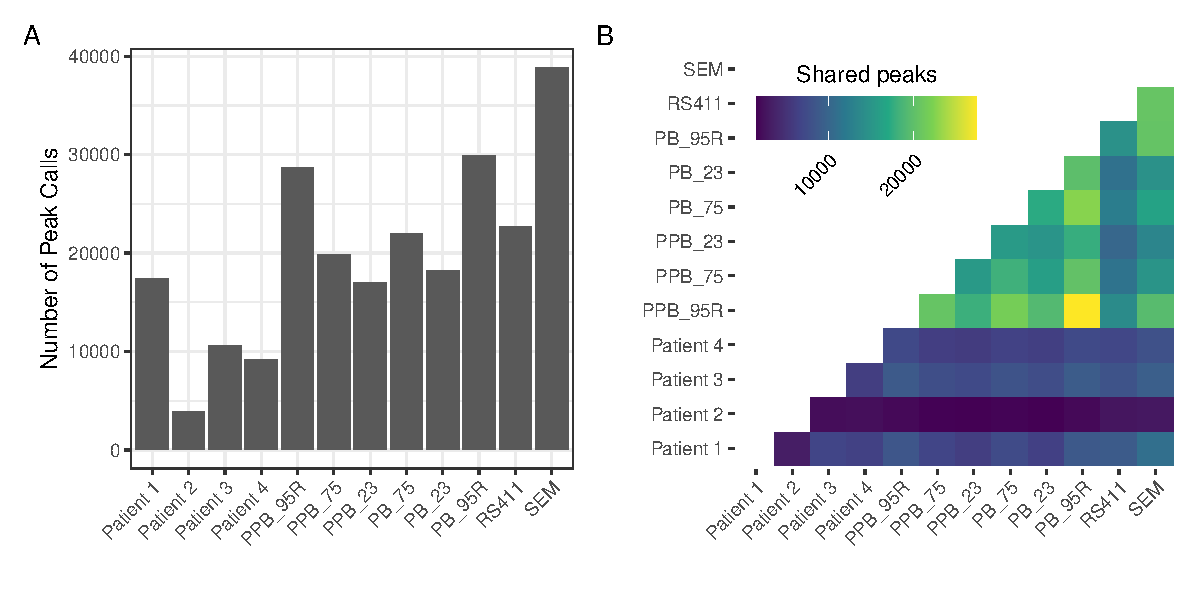
\includegraphics[width=\textwidth]{plot/ch5/mll_redo_shared_peaks.pdf}
    \caption{Peak calling of MLL-AF4 and B Cell Precursor cells with LanceOTron. A. Raw number of peak calls per cell. B. Number of shared peak calls between pairs of cells.}
    \label{fig:mll_peak_calls}
\end{figure}

% These numbers are out-dated. Not top priority to redo this. It doesn't really matter and would be similar in any case.
To justify this approach and the necessity of removing blacklisted regions, we perform the entire LDA analysis using unfiltered data, inferred topic loadings not shown. We performed region selection using the top 100, 250, and 500 regions in each topic for $k=5, \ldots, 10$ topics and found the strict overlap between the identified regions and those identified as being a part of either the ENCODE blacklist, or the ENCODE blacklist plus our custom MLL-AF4 blacklist (\Cref{fig:mll_bl_olap}). Overall, between 20.1\% and 48.8\% of the selected regions for different values of $k$ and the thresholds overlapped with ENCODE blacklisted regions. Between 51.1\% and 74.5\% of the same additionally overlapped with the custom made MLL-AF4 blacklist. 
This is compared to an overall overlap of 5998 ENCODE blacklist regions from 249903 total regions for the analysis (2.4\%) and 83434 total regions overlapping with the MLL-AF4 blacklist (33.3\%). \todo{These are from the bigwig\_merged.bed which has duplicates of the regions, so the numbers here are inflated, total is only around 63k so the others should be correspondingly less}
The blacklisted regions were therefore over-represented in the keyword regions, as expected. This analysis reaffirms the need to filter blacklisted regions.

\begin{figure}
    \centering
    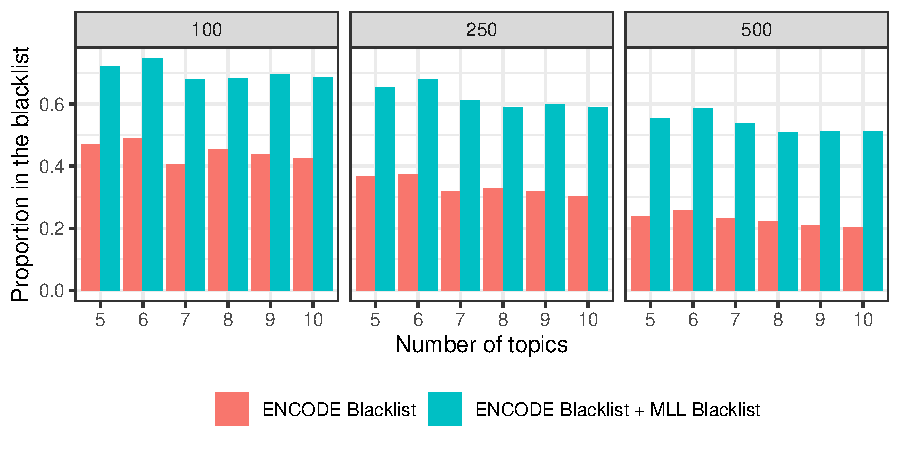
\includegraphics[width=\textwidth]{plot/ch5/mll_bl_olap.pdf}
    \caption{In an unfiltered LDA analysis of MLL-AF4 and B cell precursor cells, blacklisted regions made up the majority of identified keyword regions. Plotted is the total number of regions overlapping either of the two blacklists for a given $k$ value and the top number of regions indicated in the facet label. }
    \label{fig:mll_bl_olap}
\end{figure}

\subsection{Differential Accessibility between B cell Precursors and MLL-AF4 cells} \label{ch5:mll_diffacc}

After filtering out regions which overlapped with either the ENCODE or MLL-AF4 blacklist, we construct a count matrix using RPKM normalized read counts to test for baseline differential accessibility. We initially test for differential accessibility between the MLL-AF4 samples (Patients 1 through 4, RS411, and SEM) and the \gls{bcp} (PPB 1-3, PB 1-3). edgeR is used to identify differentially accessible regions between the two groups based on read counts. Overall, 27970 of the total 64162 regions were differentially accessible at a Q value threshold of 0.05. This is, however, too large a number to reasonably analyse in depth, so we select the top 100, 250, and 500 differentially accessible regions, all of which achieved statistical significance. We use GREAT to conduct an association analysis between these regions and pre-defined biological pathways. The background against which enrichment should be calculated is set to be union of all peak regions from the samples, in order to mitigate the inherent bias of analyzing accessible regions in the genome. All three subsets were enriched for Gene Ontology pathways, including peptidyl-threonine phosphorylation (4.97 fold enrichment, Q = $2.0e-7$), peptidyl-threonine modification (4.31 fold enrichment, Q = 2.4e-6), peptidyl-serine phosphorylation (2.59 fold enrichment, Q = 1.85e-2) and nucleic acid phosphodiester bond hydrolysis (2.62 fold enrichment, Q = 1.67e-2). The regions were also enriched for proximity to several genes, all of which with a corrected FDR Q value lower than 0.05 are shown in \Cref{tab:table:mll_edger_genes}.  Some of these genes are of immediate interest, including RHOU which promotes adhesion of T-cell \gls{all} cells via $\beta_1$ integrin, potentially implicating the protein in known impaired transendothelial migration potential of various kinds of leukemia cells \cite{Trinidad2009, Infante2013}. It is difficult to comprehensively survey this list of genes because their relationship with the identified regions is purely statistical. We have no mechanistic reason to believe that they are truly associated with disease. 

% Top 100, 250, and 500 motif enrichment maybe? Where are the regions?
\begin{table}

    \centering
    \begin{tabular}[t]{llr}
    \toprule
    Gene & FDR Q Value & Fold Enrichment\\
    \midrule
    REXO1L1P & 1.41e-33 & 62.85\\ %p
    PSKH2 & 3.70e-30 & 67.37\\ 
    FOXD4L5 & 1.29e-15 & 61.60\\
    CBWD6 & 2.08e-10 & 52.50\\
    FRG2B & 4.75e-09 & 74.86\\
    \addlinespace
    RNF187 & 4.61e-09 & 51.33\\
    RHOU & 8.52e-07 & 28.52\\
    FAM27E3 & 8.54e-07 & 39.06\\
    DUX4L3 & 7.51e-06 & 128.32\\
    FOXD4L4 & 3.36e-05 & 102.66\\
    \addlinespace
    FOXD4L2 & 7.39e-05 & 29.61\\
    SERF1A & 1.94e-04 & 73.33\\
    SMN2 & 3.55e-04 & 64.16\\
    DUX4L4 & 6.23e-04 & 128.32\\
    SPATA31A5 & 2.12e-03 & 42.77\\
    \addlinespace
    ANKRD30B & 1.19e-02 & 28.52\\
    \bottomrule
    \end{tabular}

    \caption{\label{tab:table:mll_edger_genes}Enriched genic regions from the top 500 regions differentially accessible betwen MLL-AF4 cells and BCP using edgeR.}
\end{table}

\subsection{Topic modelling for KMT2A-AFF1 leukemia}

The focus of this chapter is an in depth investigation into using topic modelling for MLL-AF4 cells. Here, we aim to discover novel pathways that differentiate MLL-AF4 cells and normal \gls{bcp}. We do this by firstly identifying a reasonable number of topics to analyse further based on patterns in topic sharing that we observe. Secondly, we select a specific number of topics and replicate the analysis a number of times. We do this to assess the contribution of stochasticity to the inference procedure. Gibbs sampling is an approach based on Monte Carlo sampling, and as such the quality of the sampled posterior distribution can depend on the starting conditions and the convergence of the algorithm. By explicitly taking into account several repetitions of the inference algorithm we attempt to minimize the effect of chance on identified key regions. 

Similar to the above cases, peak calling is performed with LanceOTron and a score threshold of 0.5, as recommended. We construct a count matrix using the normalized read counts under each peak with BLDA as well as a one-hot encoded matrix for comparison.  Hyper-parameters alpha and beta are set for a given number of topics $k$ using Bayesian optimization and loadings are inferred using cisTopic and BLDA. 

We infer topic loadings for $k=5,\ldots,12$ topics (\Cref{fig:mll_all_topic}). The upper end of this range was chosen as the number of cells in the analysis. Increase in topic number above this point are of questionable utility, as they force more structure on the data than is present naturally.  In both the OHE and BLDA approaches, topics are identified that differentiate between the MLL-AF4 and \gls{bcp} cells. However, the topics identified by BLDA tend to be more specific, loading onto some specific cells like Patients 1 and 2, SEM/RS411, PPB, or PB predominantly. No such structure is identified in the cisTopic (right hand) case. For all values of $k$ however, at least one topic is identified for the OHE case which is predominantly active in the MLL-AF4 cells over the \gls{bcp}.

\begin{figure}
    \centering
    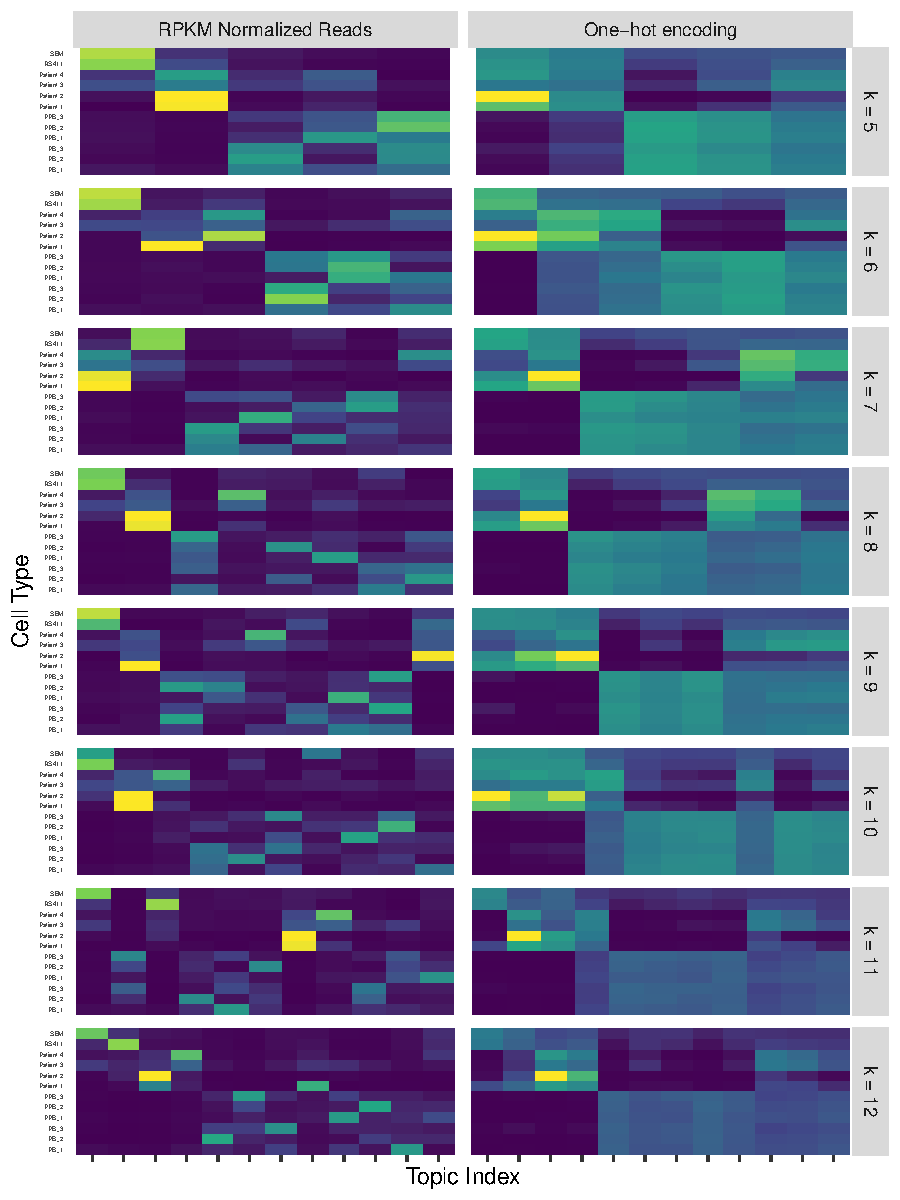
\includegraphics[width=\textwidth]{plot/ch5/mll_redo_topic_mtx.pdf}
    \caption{Inferred topic loadings for $k = 5, \ldots, 12$ topics comparing MLL-AF4 cells to B cell precursors. RPKM normalised refers to the count matrix used to infer the topic loadings by BLDA, while one-hot encoding simply annotates which regions are called as peaks by LanceOTron. Topic loadings are normalised such that the sum of all topics within a cell equals one.}
    \label{fig:mll_all_topic}
\end{figure}

Higher values of $k$ appear to impose too much structure on the data. This is evident for the BLDA case, which identifies one topic enriched for each cell type (except patient 2) at $k=12$. The OHE case interestingly deals with the over-parameterization problem differently, prefering to retain the structure seen in lower values of $k$ but assign many different topics with very low loadings within these groups. Though neither of these results are unexpected, the level of granularity for BLDA and non-specificity for OHE make it difficult to study the co-accessible regulatory elements shared between similar cell types. For that reason, we primarily are interested in the analyses for smaller values of $k$.

We select the simplest model for further analysis. We base our decision on the extremely specific topic loadings identified in the BLDA case (a single topic representing the cell lines, another involved in patients, with some sharing between them) as well as the common structure identified in PB cells separate from PPB cells with a single topic explaining the shared accessibility profile between them both. We repeat the analysis ten times for both BLDA and OHE. 

\begin{figure}
    \centering
    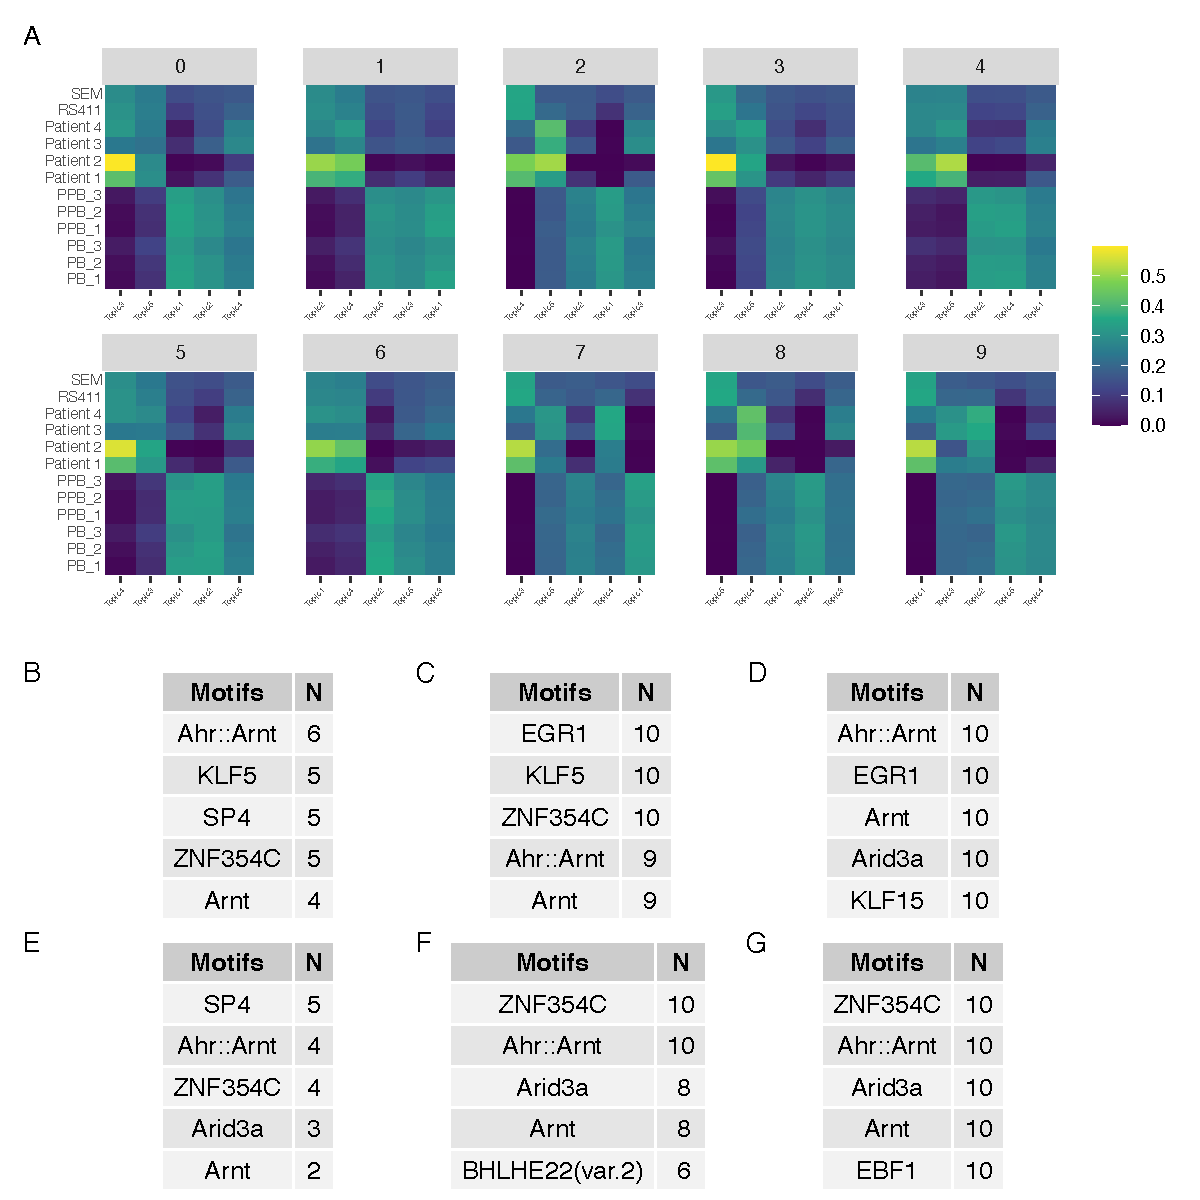
\includegraphics[width=\textwidth]{plot/ch5/mll_redo_dummy_reps.pdf}
    \caption{Ten replicates of topic modelling using one-hot encoded input. A. Inferred topic loadings on each of the samples for all 10 replicates, sorted by median topic activation. B, C, and D show the top 5 motifs identified in $N$ of the replicates in the top 100, 250, and 500 regions of manually annotated MLL-AF4 specific topics. E, F, and G show an equivalent for BCP specific topics.}
    \label{fig:mll_redo_topics}
\end{figure}

\subsubsection{Five topic one-hot encoding replication}

The $k=5$ OHE analysis consistently identifies at least one topic which is active in all of the MLL-AF4 cells and none of the \gls{bcp} samples (\Cref{fig:mll_redo_topics}). Patient 2 is usually the most active representative of this group within that topic. Some replicates (i.e. replicates 2, 5, 6, 7, 8, 9) also find topics active in all of the \gls{bcp} and few of the MLL-AF4 samples. There is no obvious substructure within the \gls{bcp} samples.  We manually annotate each topic as "enriched in MLL-AF4 cells", "enriched in \gls{bcp}", or neither and perform enrichment for each of the two specific sets relative to the other topics.  Motifs found in the MLL-AF4 speciifc topics in the top 100, 250, and 500 regions include SP4, KLF5, EGR1, and KLF15 (\Cref{fig:mll_redo_topics}B, C, D). Ahr::Arnt, ZNF354C, Arid3a, and Arnt are identified but found broadly between MLL-AF4 and \gls{bcp} regions.  The latter were additionally enriched for BHLHE22 and EBF1 which is a marker for B cell lineage commitment \cite{Infante2013} along with PAX5 which is occasionally identified in \gls{bcp} specific regions (data not shown). The list of motifs presented is reasonably unspecific, though there is evidence that EGR1 has deep functional relationships with many hematological malignancies including \gls{all} \cite{Tian2016}. The fact that there is at least one known system specific transcription factor whose motif is enriched for each set of samples is reassuring.  It is additionally reassuring that these important motifs were identified in each of the ten replicates in their respective sets.  Even in this low-resolution OHE setup, the technique has some power to robustly identify relevant biology across replicates.

\begin{figure}
    \centering
    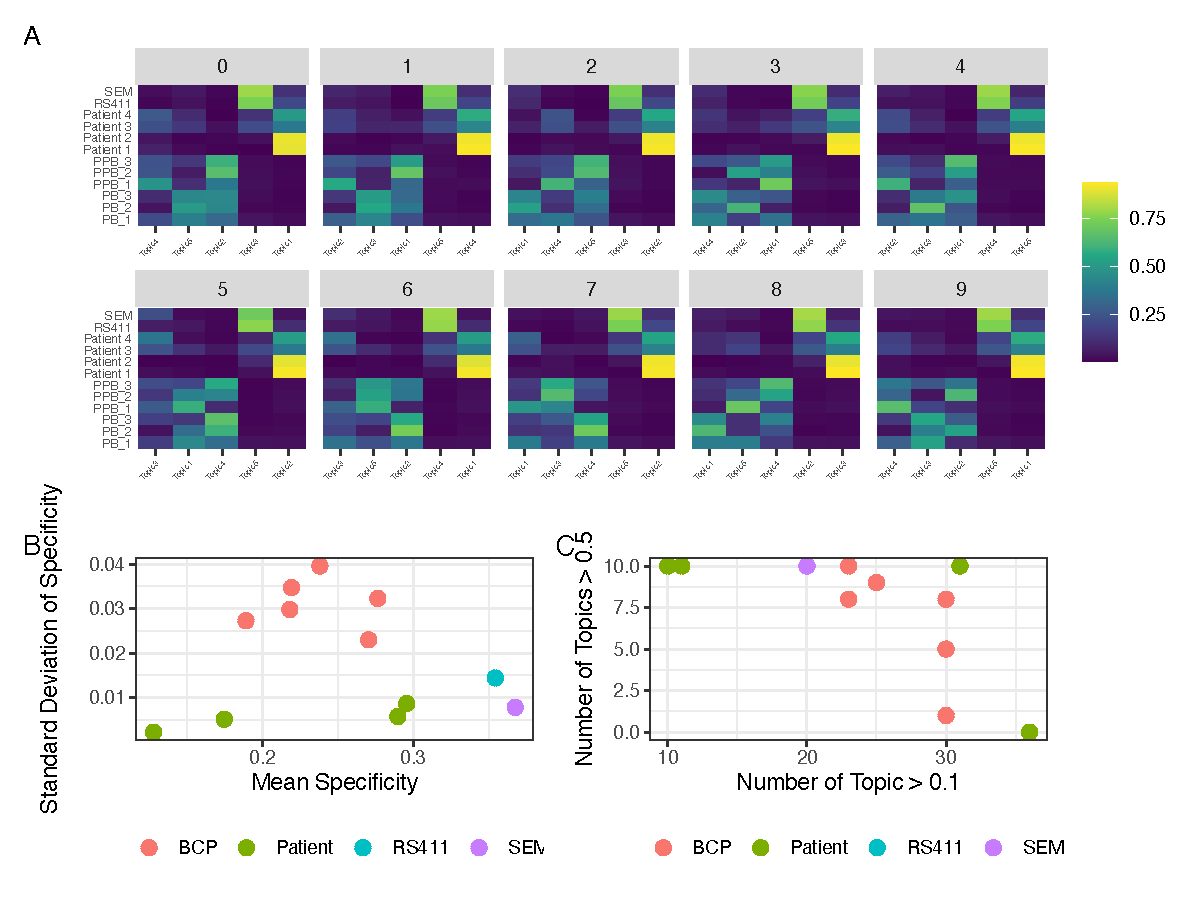
\includegraphics[width=\textwidth]{plot/ch5/mll_redo_reps_bigwig.pdf}
    \caption{Ten replicates of topic modelling using RPKM normalized input, aka BLDA. A. Inferred topic loadings for each of the 12 samples and all 10 replicates, sorted by standard deviation of topic loading. B. Mean versus standard deviation of specificity, here defined as the contribution of the most enriched topic to that sample divided by the sum of that topics enrichment to all other samples. Averaged over replicate. C. The number of instances where a sample has a topic identified above a loading value of 0.1 versus the number of instances where any topic is annotated above 0.5. Values represent contribution of a particular topic to a particular cell, such that the sum of topic loadings within a particular cell equals 1.}
    \label{fig:mll_reps}
\end{figure}

\subsubsection{BLDA replication with five topics}

The inferred topic loadings in the BLDA case are also reproducible across replicates (\Cref{fig:mll_reps}A). In each of the 10 replicates, one topic loads preferentially onto Patients 1 and 2, and to a lesser degree onto patients 3 and 4. Another loads preferentially onto RS411 and SEM. The remainder are somewhat divided between a common co-accessibility program amongst all samples (i.e. topic 3 in replicate 5), specifically loading onto PPB (i.e. topic 5 in replicate 6), or PB (Topic 5 in replicate 0). In general, each of the replicates has at least one topic that falls into each of these categories, though the loadings onto the \gls{bcp} are less consistent than the MLL-AF4 cells. The topics loading onto RS411 and SEM were highly specific to those two samples, in contrast to the BCPs whose specificity was much lower, and additionally much more variable (\Cref{fig:mll_reps}B).  The BCPs additionally had many topics annotated to them at low levels, but very few with a higher annotation level of 0.5 (\Cref{fig:mll_reps}C).  This is in contrast to Patients 1 and 2, who had both a large number of highly specific topics across the replicates, and also a very low number of non-specific topics.  From this we conclude that similar topics are able to be found consistently across replicates.  

Having established a high degree of specificity for individual topics to the expected annotations of the samples, we investigate the regions making up the topics. We briefly focus on a single replicate, indexed as 0 in \Cref{fig:mll_reps}. An interesting avenue for exploration is the degree to which the topics are made up of similar regions. If they were, it would represent a shared core of co-accessible elements. The alternative, of completely separate underlying regions, is equally interesting. An understanding of the region-topic distribution over cell types will aid in the interpretation of the key regions for particular topics. We transform each region-topic vector to $Z$-scores by subtracting the mean and dividing by the standard deviation of the distribution, and count the number of regions with a $Z$-score over 3 (98.8 percentile of a theoretical standard normal distribution) in each of the topics (diagonal of \Cref{fig:mll_region_sharing}A). We additionally count the regions with a $Z$ score of 3 or higher in both of two different topics and find generally low region sharing overall, except in the case of topics 2 and 5 where 330 regions were enriched for both(off-diagonal elements of \Cref{fig:mll_region_sharing}A). Topics 2 and 5 in this replicate were enriched for PB cells and all BCP respectively. The regions selected as a part of this set had higher read counts in BCP samples than MLL-AF4 samples (\Cref{fig:mll_region_sharing}B).  This indicates a high degree of co-accessibility between important regions in PB and PPB cells. In contrast to this, few regions were shared between the two MLL-AF4 topics. The regions with topic 1 loadings over a $Z$ score of three were more accessible in the patient samples, though this was not a statistically significant difference (\Cref{fig:mll_region_sharing}C). However, the small number of important regions for the RS411/SEM topic were more accessible in these cell types (\Cref{fig:mll_region_sharing}).

\begin{figure}
    \centering
    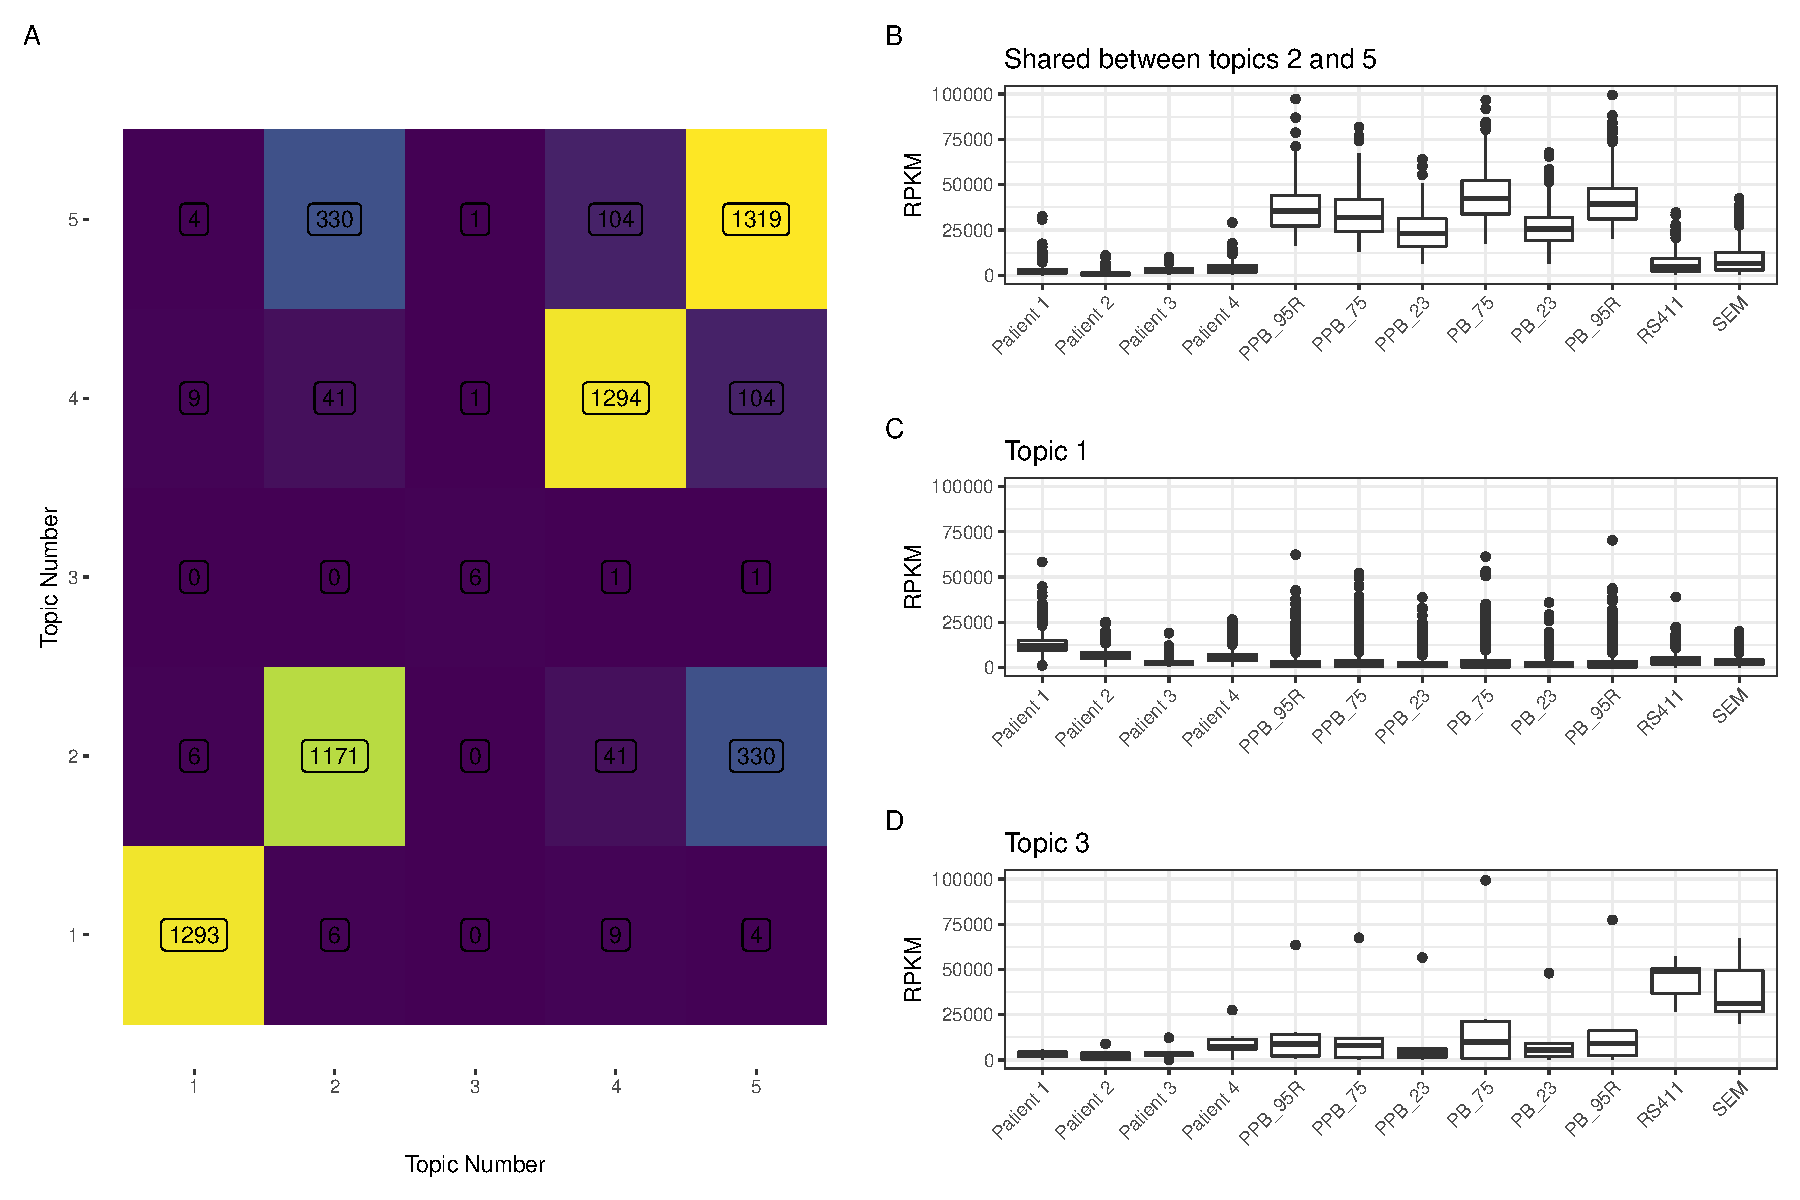
\includegraphics[width=\textwidth]{plot/ch5/mll_bigwig_region_sharing_plot_rep0.pdf}
    \caption{Regions highly annotated on each of the five topics in replicate 0 for the BLDA topic modelling. A. Region-topic loadings were converted to Z scores by subtracting the mean of the distribution and dividing by the standard deviation. Regions with a $Z$ score of 3 or more were selected, and the number of shared highly loaded regions is plotted. The number identified per topic is plotted on the diagonal. B. RPKM values for the 330 regions highly loaded for both topics 2 and 5. In this replicate, these topics were enriched in BCPs. C. RPKM values for regions highly loaded with topic 1, which primarily loads onto patient samples. D. RPKM values for the 6 regions highly loaded with topic 3, which is enriched in RS411 and SEM samples.}
    \label{fig:mll_region_sharing}
\end{figure}

\subsubsection{Sample-specific key-word regions across replications}

We sought to understand how reproducibly these regions were identified between replicates. 
Regions robustly identified as being associated with a topic that loads highly onto a desirable set of samples represent key candidates for further investigation.
We identified the top 100, 250, and 500 regions for each topic in each replicate, and found how many of these regions are shared between 8, 9, or all of the replicates (\Cref{fig:mll_region_repro}A). Patients have the highest key-word topic reproducibility across replicates, with 76 of the top 100 identified in every single replicate. The patient group has the lower number of unique regulatory elements identified for any threshold (\Cref{fig:mll_region_repro}B). Amongst the 76 reproducibly identified regions, average expression is almost threefold higher in patients than the remainder of samples (mean of patients = 11321.8, mean of other = 4291.5, Student's $T$-test $P$ value for difference < 2.2e-16). These regions therefore represent a prioritized set that is both important for the highly-specific topic modelling approach and identified in each of the ten replicates. 

Deriving some idea of functional characteristics from an abitrary set of genomic regions is difficult. Evolutionary conservation, biochemical properties such as histone modifications, and studying genetic mutations can all lend some degree of credibility linking a collection of regions to a particular pathway of interest \cite{Kellis2014}. Within the context of this sample, understanding the role of these regions is additionally confounded by the fact that they are derived from blastic, malignant cancer cells. Practically, this means that they may contain somatic mutations not represented in the reference panel. At present, there is no reliable, published, method for calling mutations from peak-based NGS experiments. Even if this data were available, it would be difficult to differentiate between accessibility as a consequence of cellular environment and differential evolution from that caused by genetic differences. The interpretation of the functional role of regions identified herein is hampered by a lack of functional validation due to the timelines imposed on this thesis.  

\begin{figure}
    \centering
    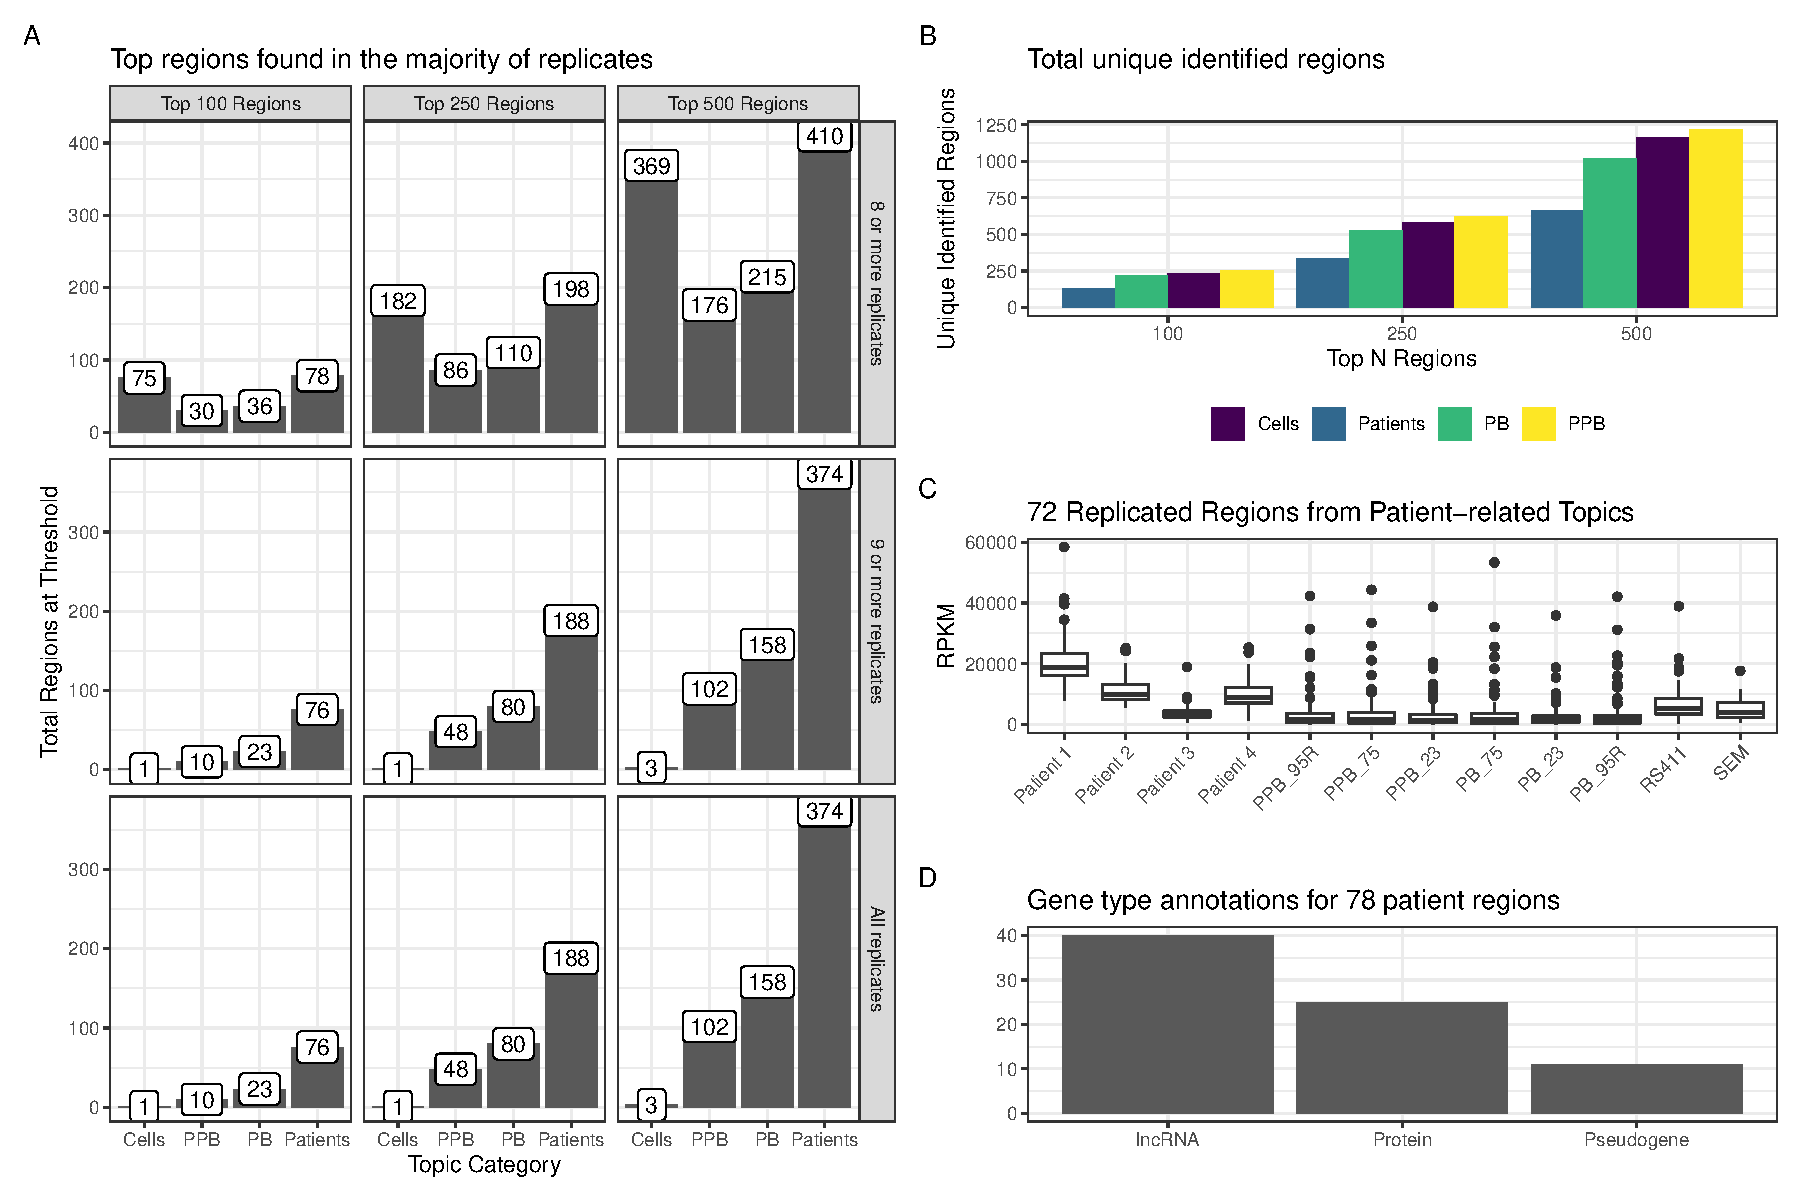
\includegraphics[width=\textwidth]{plot/ch5/mll_top_regions_bigwig.pdf}
    \caption[A subset of patient specific regions are highly reproducible across replicates and are enriched for lncRNA genes.]{A subset of patient specific regions are highly reproducible across replicates and are enriched for lncRNA genes. A. For each of the 100, 250, or 500 top regions per manually annotated sample specific topic, the number of regions occuring in eight or more, nine or more, or all of the ten replicates is plotted. B. The intersection of all regions identified across replicates for each set of sample-specific topics. C. RPKM profile for the 76 regions identified in A as being highly reproducible. D. Gene type annotation from refseq for closest annotated genes for the same regions.}
    \label{fig:mll_region_repro}
\end{figure}

\subsection{Annotating reproducibly identifiable patient-related regions}

We begin our characterization of these regions by finding their closest annotated gene body. 32 of the 76 regions lie directly within genic regions. The remainder tend to be found within 50kb of the nearest gene, but the distance is highly variable and some regions are as far as 200kb from their closest gene (\Cref{fig:mll_lnc}A). This distance distribution fits well to our expectations if the regions represented inter-genic enhancer elements.  The closest annotated genes are, interestingly, \glspl{lnc}, and are found in a much higher frequency than expected in 76 randomly samples genes (\Cref{fig:mll_lnc}B,C). Though this result is suggestive, \glspl{lnc} are very challenging to correctly annotate, with efforts being confounded by both technical artifacts and methodological complications \cite[see Figure 1 for an overview of challenges associated with lncRNA annotation]{Cao2018}. There is, however, growing evidence that cancer cells, including leukemic blasts, may hijack the large and poorly understood lncRNA transcriptome to influence differentiation, energy metabolism, malignant proliferation, apoptosis, and the drug resistance of leukemia cells \cite[Table 1]{Gao2020}. It is possible, therefore, that the regions identified represent \glspl{cre} influencing the expression of functional lncRNAs involved in each individual patient's leukemia. However, none of the lncRNAs identified match with those in Table 1 of \textcite{Gao20202}, so their potential functions will remain the subject of further investigation.

\begin{figure}
    \centering
    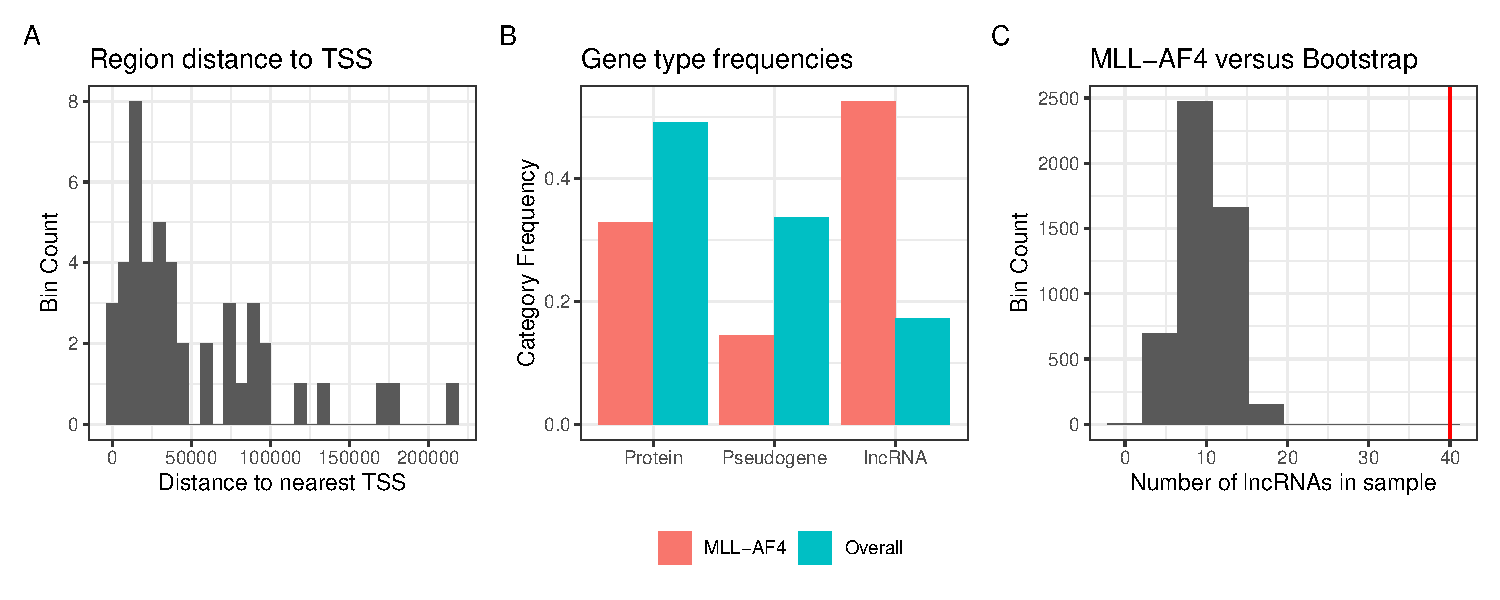
\includegraphics[width=\textwidth]{plot/ch5/mll_lnc.pdf}
    \caption{MLL-AF4 regions compared to reference genes. A. Distance of the 76 reproducible patient regions to their nearest annotate TSS, minus the regions which are sitting in genic regions. B. Frequencies of gene categories in refSeq versus the sample of closest patient genes. C. Frequency of lncRNAs in 5000 random samples of 76 regions from refSeq, showing that the observed frequency of lncRNA is in the far tail of this distribution.}
    \label{fig:mll_lnc}
\end{figure}

\subsubsection{Histone modifications and transcription factor binding in the patient-related regions}

Histone proteins within nucleosomes may be post-translationally modified by the addition of several chemical groups which collectively serve to regulate transcription and the recruitment of transcription factors. The presence of specific histone modifications at a particular location of the genome can be determined experimentally using \gls{chip}, where peak regions give an estimate of the presence or absence of a particular modification. There are many histone modifications, and their combinatorial method of action makes it difficult to interpret the exact ramifications of their presence \cite{T2001}. Previously, a small number of important histone modifications and transcription factor binding sites were characterized in these samples (see Methods).  

We called peaks on each of the ChIP-seq tracks using LanceOTron and intersected the peaks with the reproducible set of patient regions. We additionally drew 1000 random samples from the set of accessible regions used in this section, creating an empirical P-value, to understand the relative enrichment of these ChIP-seq signals versus the genomic background of accessible sequence. Within the available ChIP-seq data, regions are relatively enriched for H3K27ac, H3K4me1, and H3K4me3 (\Cref{table:mll_chip}). They are depleted in K379me2, and there is evidence that we see more binding of MLL to these regions than we would expect by chance, especially in patient 11911, where we additionally see increased binding of AF4, PAF1c, and RUNX1. The relative abundance of H3K27ac and H3k4me1 indicate that these elements may be acting as enhancers. However, it is not clear whether the high abundance of PAF1c, RUNX1, and MLL marks are due to general enrichment in enhancer regions or are somehow associated with these regions functionally. As patient 11911 is the only available sample with all of these chromatin marks and transcription factors available, we elect to study this patient specifically. We create a set of putative enhancer elements by selecting 18101 regions from the total 64162 accessible regions that overlap with both H3K27ac and H3K4me1 peaks. We then perform a similar analysis to before, selecting 5000 sets of 76 regions at random and observing the proportion of the putative enhancer elements that are additionally bound by MLL, AF4, PAF1c, and RUNX1. The resulting distributions show that none of the 5000 random samples are as highly enriched for MLL, PAF1c, or RUNX1 as the reproducible patient regions (\Cref{fig:mll_enhancer_overlap}). MLL binding is enriched by approximately 50\% over the mean of the distribution (67 versus 44.8), RUNX1 binding is 63\% higher than the mean (48 versus 29.3), and PAF1c is enriched by nearly 70\% (52 versus 30.6). We discuss the relevance of these transcription factors in the Discussion section. 

\begin{figure}
    \centering
    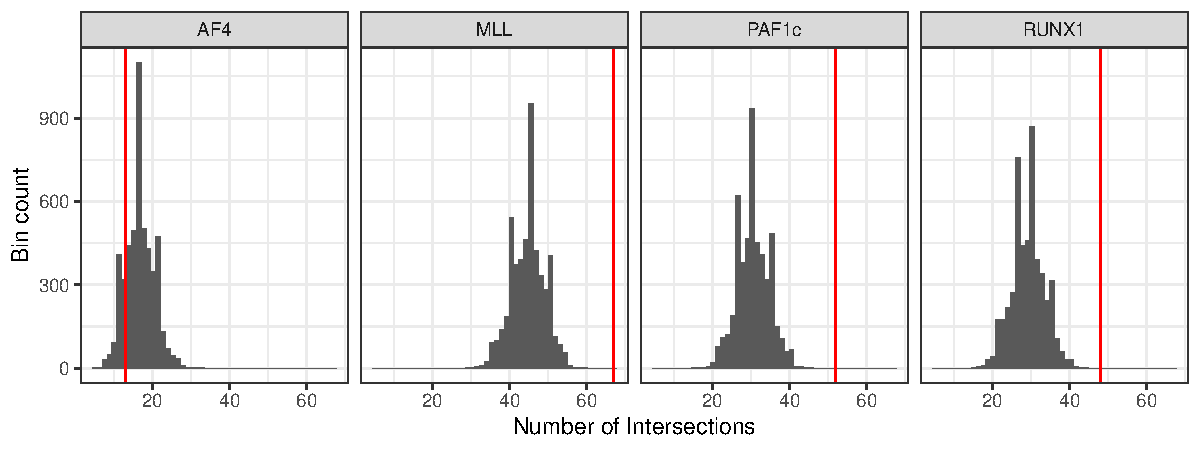
\includegraphics[width=\textwidth]{plot/ch5/mll_enhancer_overlap.pdf}
    \caption{Number of intersections between 76 randomly selected putative enhancer sites (accessible regions which overlapped with both H3K4me1 and H3K27ac chromatin peaks) in 5000 random samples compared to the observed quantities in the reproducible patient regions (plotted in red as a vertical line).}
    \label{fig:mll_enhancer_overlap}
\end{figure}

\begin{figure}
    \centering
    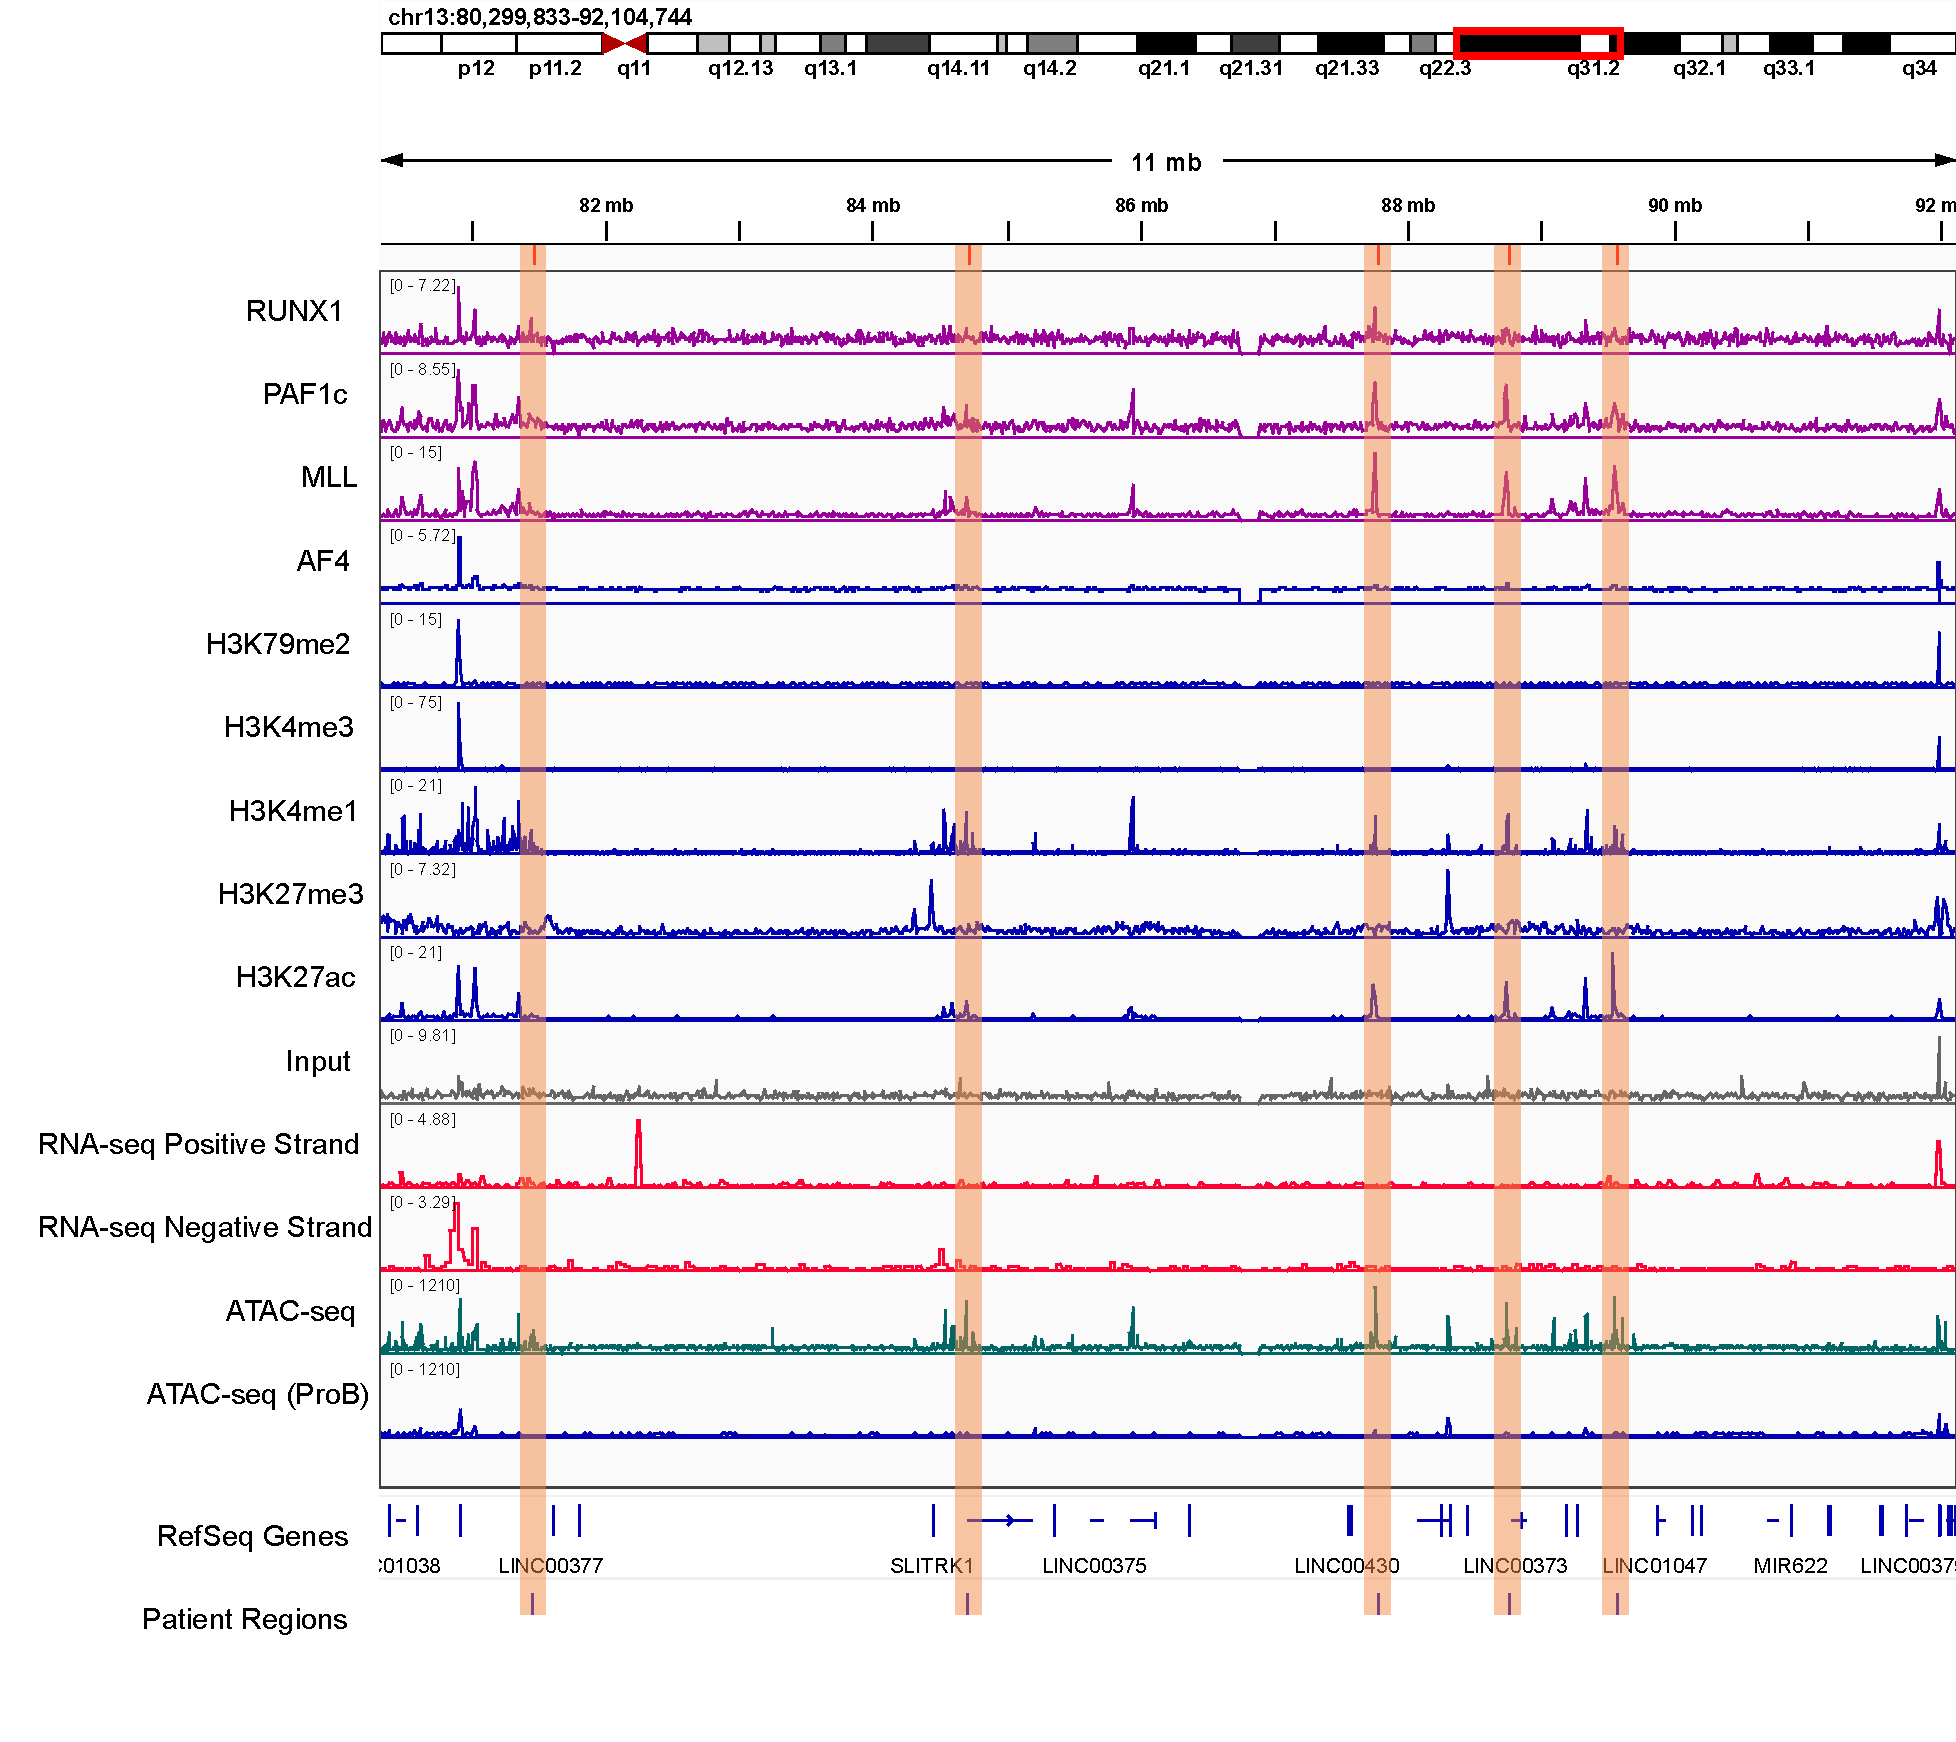
\includegraphics[width=\textwidth]{plot/ch5/enhancer_cluster.pdf}
    \caption{Coverage tracks for ChIP-seq marks, RNA-seq, and ATAC-seq for patient 11911 as well as PB cell for comparison. Five regions are in close promiximity to each other, each marked with H3K4me1, H3K27ac, MLL, and PAF1c. Regions of interest are highlighted in orange, with the highlight extending slightly beyond their borders for visual clarity.}
    \label{fig:mll_enhancer_cluster}
\end{figure}


\begin{table}

    \centering
    \tiny
    \begin{tabular}[t]{llllllllll}
    \toprule
    Patient ID & H3K27ac & H3K4me1 & H3K4me3 & H3K79me2 & MLL & AF4 & H3K27me3 & PAF1c & RUNX1\\
    \midrule
    26754 & 57 (0) & 60 (0) & 31 (0) & 2 (0.968) & 42 (0) & 4 (0.631) &   &   &  \\
    11911 & 66 (0) & 72 (0) & 32 (0) & 2 (0.975) & 67 (0) & 13 (0.004) & 1 (0.933) & 52 (0) & 48 (0)\\
    27800 & 60 (0) & 61 (0) & 38 (0) & 3 (0.956) &   &   &   &   &  \\
    25911 & 23 (0) &   &   &   & 24 (0) &   &   &   &  \\
    \bottomrule
    \end{tabular}
    \caption{ChIP-seq peak overlaps with reproducible patient regions, with the proportion of overlaps from 1000 random draws from all accessible regions in brackets. }
    \label{table:mll_chip}
    \end{table}


\begin{table}[]
    \tiny
    \begin{tabularx}{\textwidth}{lllX}
    \toprule
    Region                                     & Function                   & Gene        & Cell line reference                                                             \\ \midrule
    chr1:239881927-239883919                   & Promoter                   & CHRM3-AS2   &                                                                                 \\
    \multirow{4}{*}{chr2:133023823-133025309}  & \multirow{4}{*}{Enhancer}  & AC098826.5; & GM19238;                                                                        \\
                                               &                            & CDC27P1;    & GM19238,Pancreatic\_islet;                                                      \\
                                               &                            & GPR39;      & Pancreatic\_islet;                                                              \\
                                               &                            & LYPD1       & Pancreatic\_islet                                                               \\
    \multirow{4}{*}{chr3:97628722-97630587}    & \multirow{4}{*}{Enhancer}  & ARL6;       & HT29;                                                                           \\
                                               &                            & AC110491.1; & HT29;                                                                           \\
                                               &                            & CRYBG3;     & HT29,PC3,th1,Thymus;                                                            \\
                                               &                            & MINA        & HT29,Mesendoderm,NB4,PC3                                                        \\
    \multirow{9}{*}{chr3:160554953-160556142}  & \multirow{9}{*}{Enhancer}  & IFT80;      & HT29;                                                                           \\
                                               &                            & RP11;       & HT29,NB4;                                                                       \\
                                               &                            & TRIM59;     & HT29;                                                                           \\
                                               &                            & SCARNA7;    & HT29;                                                                           \\
                                               &                            & ARL14;      & HT29;                                                                           \\
                                               &                            & RP11;       & HT29,NB4;                                                                       \\
                                               &                            & PPM1L;      & HT29,NB4;                                                                       \\
                                               &                            & RP11;       & HT29,NB4;                                                                       \\
                                               &                            & NMD3        & NB4                                                                             \\
    \multirow{10}{*}{chr3:190303470-190305623} & \multirow{10}{*}{Enhancer} & IL1RAP;     & HFF,hMADS-3,HT29,Keratinocyte,MCF10A,\newline melanoma,Mesendoderm,NB4,PC3,T98G,ZR75-30; \\
                                               &                            & GCNT1P3;    & hMADS-3,Keratinocyte,MCF10A,melanoma,NB4;                                       \\
                                               &                            & 7SK;        & hMADS-3,Keratinocyte,MCF10A,melanoma,NB4;                                       \\
                                               &                            & MTAPP2;     & HT29,Keratinocyte,Mesendoderm,T98G;                                             \\
                                               &                            & CLDN1;      & HT29,Keratinocyte,MCF10A,PC3;                                                   \\
                                               &                            & LEPREL1;    & Keratinocyte,MCF10A,Mesendoderm;                                                \\
                                               &                            & CLDN16;     & Keratinocyte,NB4;                                                               \\
                                               &                            & CCT6P4;     & Keratinocyte,NB4;                                                               \\
                                               &                            & TMEM207;    & NB4;                                                                            \\
                                               &                            & RP11        & NB4                                                                             \\
    \multirow{8}{*}{chr4:54721244-54722456}    & \multirow{8}{*}{Enhancer}  & RP11;       & HFF,ZR75-30;                                                                    \\
                                               &                            & LNX1;       & HFF;                                                                            \\
                                               &                            & RP11;       & HFF,ZR75-30;                                                                    \\
                                               &                            & CHIC2;      & HFF,ZR75-30;                                                                    \\
                                               &                            & RP11;       & HFF,ZR75-30;                                                                    \\
                                               &                            & PDGFRA;     & HFF;                                                                            \\
                                               &                            & RPL21P44;   & ZR75-30;                                                                        \\
                                               &                            & MORF4L2P1   & ZR75-30                                                                         \\
    \multirow{3}{*}{chr4:177823634-177824977}  & \multirow{3}{*}{Enhancer}  & SPCS3;      & HFF;                                                                            \\
                                               &                            & RP11;       & HFF,LHCN-M2,SK-N-SH\_RA;                                                        \\
                                               &                            & NEIL3       & Keratinocyte,MCF10A                                                             \\
    chr5:82663769-82665217                     & Enhancer                   & TMEM167A    & ZR75-30                                                                         \\
    \multirow{3}{*}{chr5:119723091-119724865}  & \multirow{3}{*}{Enhancer}  & PRR16;      & HFF;                                                                            \\
                                               &                            & CTD;        & HFF,LHCN-M2;                                                                    \\
                                               &                            & RP11        & melanoma                                                                        \\
    \multirow{2}{*}{chr6:141130170-141131796}  & \multirow{2}{*}{Enhancer}  & RP3;        & ME-1;                                                                           \\
                                               &                            & RP11        & ME-1                                                                            \\
    chr6:161161634-161163661                   & Enhancer                   & PLG         & GM12891,Namalwa                                                                 \\
    chr7:11870320-11872428                     & Promoter                   & THSD7A      &                                                                                 \\
    chr7:81474664-81476523                     & Enhancer                   & MIR1255B1   & NB4                                                                             \\
    \multirow{3}{*}{chr8:77492793-77494807}    & \multirow{3}{*}{Enhancer}  & MRPL9P1;    & ESC\_neuron,SK-N-SH\_RA;                                                        \\
                                               &                            & ZFHX4;      & ESC\_neuron;                                                                    \\
                                               &                            & RP11        & ESC\_neuron,SK-N-SH\_RA                                                         \\
    chr9:42018481-42020192                     & Promoter                   & \multicolumn{2}{l}{LOC102724238,LOC554249,KGFLP2}                                             \\
    chr9:46686996-46688539                     & Promoter                   & \multicolumn{2}{l}{KGFLP1,LOC554249,LOC102724238}                                             \\
    \multirow{8}{*}{chr10:33654161-33655412}   & \multirow{8}{*}{Enhancer}  & AK3P5;      & FT246,HFF,hMADS-3,HT29,LHCN-M2,ZR75-30;                                         \\
                                               &                            & RP11;       & FT246,FT33,HFF,hMADS-3,HT29,Keratinocyte,LHCN-M2,ZR75-30;                       \\
                                               &                            & RP11;       & FT246,FT33,HFF,hMADS-3,HT29,Keratinocyte,LHCN-M2,ZR75-30;                       \\
                                               &                            & ITGB1;      & FT246,FT33,HFF,hMADS-3,HT29,Keratinocyte,LHCN-M2,ZR75-30;                       \\
                                               &                            & RP11;       & FT246,FT33,HFF,hMADS-3,HT29,Keratinocyte,LHCN-M2,ZR75-30;                       \\
                                               &                            & RP11;       & FT246,FT33,HFF,hMADS-3,HT29,Keratinocyte,LHCN-M2,ZR75-30;                       \\
                                               &                            & NRP1;       & FT246,FT33,HFF,hMADS-3,LHCN-M2;                                                 \\
                                               &                            & AL353600.1  & hMADS-3                                                                         \\
    chr10:58119756-58122125                    & Promoter                   & ZWINT       &                                                                                 \\
    chr12:24531253-24532422                    & Enhancer                   & BCAT1       & hMADS-3,Mesendoderm                                                             \\
    \multirow{2}{*}{chr13:54602807-54604709}   & \multirow{2}{*}{Enhancer}  & LINC00458;  & Mesendoderm;                                                                    \\
                                               &                            & RPL13AP25   & Mesendoderm                                                                     \\
    chr13:84710151-84712348                    & Promoter                   & LINC00333   &                                                                                 \\
    \multirow{5}{*}{chr13:103658908-103660657} & \multirow{5}{*}{Enhancer}  & TPP2;       & GM19238,GM19239,HFF,Namalwa;                                                    \\
                                               &                            & KDELC1;     & GM19238,GM19239,HFF,Namalwa;                                                    \\
                                               &                            & BIVM;       & GM19238,GM19239,HFF,Namalwa;                                                    \\
                                               &                            & ERCC5;      & GM19238,GM19239,HFF,Namalwa;                                                    \\
                                               &                            & TEX30       & HFF,Namalwa                                                                     \\
    \multirow{2}{*}{chr14:38593423-38595439}   & \multirow{2}{*}{Enhancer}  & CTD;        & Mesendoderm;                                                                    \\
                                               &                            & SSTR1       & Mesendoderm                                                                     \\ \cmidrule(l){1-4} 
    \end{tabularx}
    \caption{EnhancerAtlas 2.0 results for the 76 reproducibly identified patient regions.}
    \label{table:mll_enhancer}
    \end{table}



% discuss this in the discussion, don't interperet it here.

\subsubsection{Known annotations in EnhancerAtlas} 

We searched EnhancerAtlas 2.0 (Citation) for regions matching ours, and found that 17 out of the 76 regions were known enhancers, and 6 were known promoters (\Cref{table:mll_enhancer}). The functionality validated active cell types varied considerably, from enhancers for GPR39 and LYPD1 in pancreatic islet cells to more similar TMEM207 and RP11 enhancers in pro-myelotic leukemia cell line NB4. In this list as well, non-coding RNA targets are also over-represented. RP11, for example, was identified as functionally validated target of 10 of the 17 enhancers. Though RP11 represents a class of otherwise unannotated genes, rather than a protein of its own, many subtypes of RP11 are in fact non-coding RNAs (CITATION). As previously mentioned, these regions are clearly marked as putative enhancer regions, though it is not immediately obvious which genes they may be regulating. Interestingly, some regions co-occur in clusters such as the one on Chromosome 13 in \Cref{fig:mll_enhancer_cluster}. Here, five regions are found together, each marked with enhancer marks H3K4me1 and H3K27ac as well as the transcription factors MLL and PAF1c. The second of these five regions is annotated as an enhancer for TPP2, KDELC1, BIVM, ERCC5, and TEX30 in GM EBV-immortalized cells as well as a fibroblast cell line HFF-1. Whether the remainder of the enhancers are novel in the MLL-AF4 patients remains to be shown experimentally, however there is no clear accessibility in these regions for \glspl{bcp}. 


\subsection{Validation of patient-related regions within the ENCODE Consortium Blood Cell Collection}

To investigate this further, we collect all of the blood related cell types in the ENCODE consortium's list of available ATAC-seq experiments. We exclude any DNase-seq experiments due to known sysmtematic differences as well as the unproven ability of the method to transfer between accessibility protocols \cite{Klemm2019a}. Without an obvious way to show that differences between DNase-seq and ATAC-seq are not a result of modelling systematic differences, we restrict the analysis to 143 samples within the ENCODE database with available coverage tracks in BigWig format and which are annotated as being associated with the blood tissue system. This data is downloaded and peak called using LanceOTron as before, excluding regions in the ENCODE blacklist as well as the MLL-AF4 specific blacklist developed in \Cref{mll_blacklist}. We additionally use liftOver to transfer genomic coordinates from the native GRCh38 to hg19 to match the other samples' build. The dataset contained, in total, 326427 regions and 155 ATAC-seq experiments. We begin our validation by examining the previously identified regions in the entire ENCODE blood data set. Interestingly, the five regions contained in the previously described putative enhancer cluster are all most accessible in patients compared to any other cell type in the ENCODE blood cell type collection, suggesting that their function may be new in these patient samples (\Cref{fig:encode_pt_regions}). In fact, 74 of the 76 patient regions were the most accessible in patient samples, with the other two being more accessible in BCPs and MLL-AF4 cells rather than the ENCODE dataset.

\begin{figure}
    \centering
    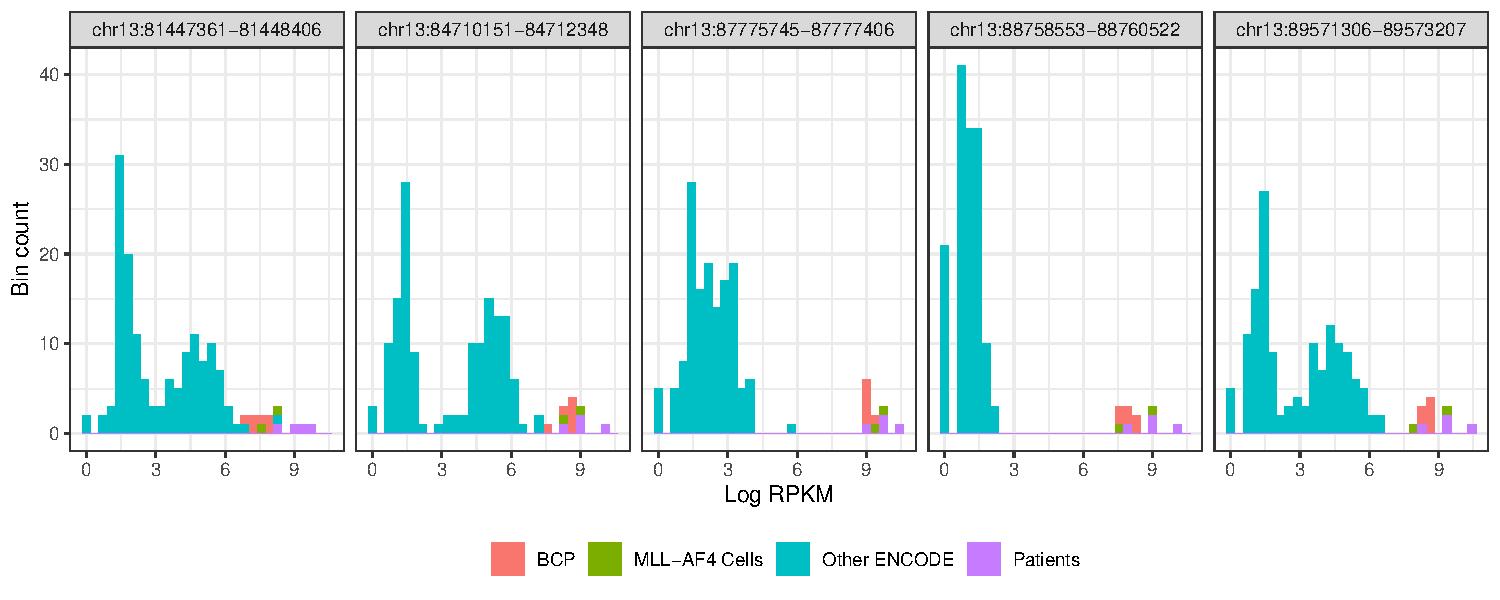
\includegraphics[width=\textwidth]{plot/ch5/pt_compared_to_encode.pdf}
    \caption{Log RPKM for five regions in a putative enhancer cluster identified through topic modelling in ENCODE blood cells versus patients and MLL-AF4 cell types.}
    \label{fig:encode_pt_regions}
\end{figure}

We perform topic modelling on the entirety of the ENCODE dataset alongside the MLL-AF4 and \gls{bcp} samples. Hyper-parameter optimization is difficult in this system, purely due to computational considerations. Therefore we select reasonable hyper-parameters based on the defaults for single-cell analyses, setting alpha to 50 and beta to 0.1, as is the recommended default for cisTopic. We run the analysis modelling $k=10,15,20,25,30$ and examine the output (\Cref{fig:encode_all}). The relative sparsity of the topic loadings above $k=15$ leads to each of the patients and BCP cells essentially being enriched for a seperate topic, which makes interpretation difficult. The $k=10$ and $k=15$ cases both model the structure of the system well, however, especially amungst the most closesly related cell types (left-hand side of \Cref{fig:encode_zoom}). The one-hot encoding does not decifer any different structure within the MLL-AF4 and BCP population for either of the two $k$ values, only loading a single topic strongly and a second weakly to the entirety of the set (right-hand side of \Cref{fig:encode_zoom}). Some interesting discrepencies between the $k=10$ and $k=15$ case include an active B cell topic in $k=15$ which loads weakly onto BCP cells but not MLL-AF4 samples. Additionally, patients 3 and 4 share a topic with MLL-AF4 cell lines in the $k=10$ analysis but not in the $k=15$ version.  


\begin{figure}
    \centering
    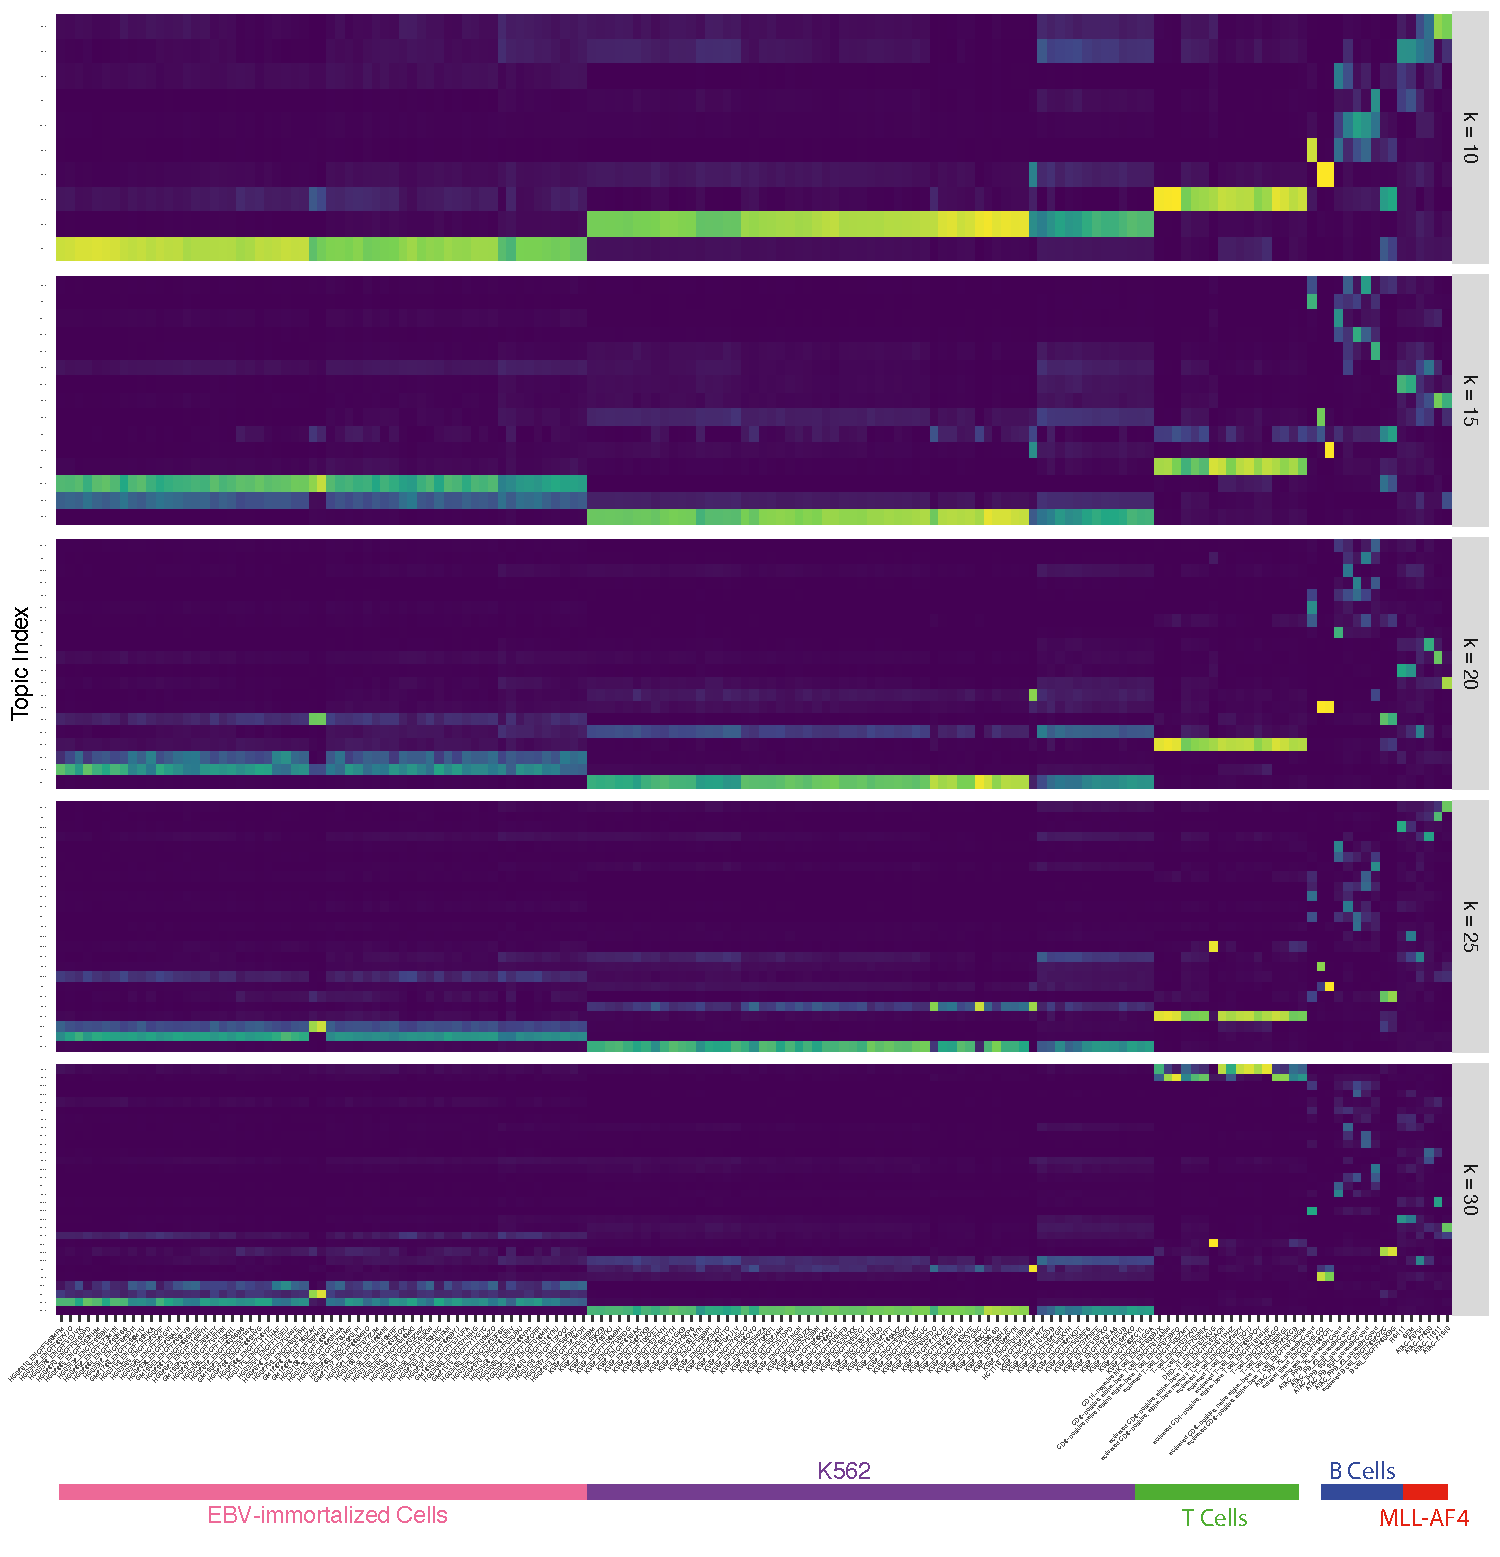
\includegraphics[width=\textwidth]{plot/ch5/mll_encode_all_topics.pdf}
    \caption{Topic modelling for ENCODE blood cell collection with MLL-AF4 and BCP samples for $k=10,15,20,25,30$. }
    \label{fig:encode_all}
\end{figure}

\begin{figure}[htbp]
    \centering
    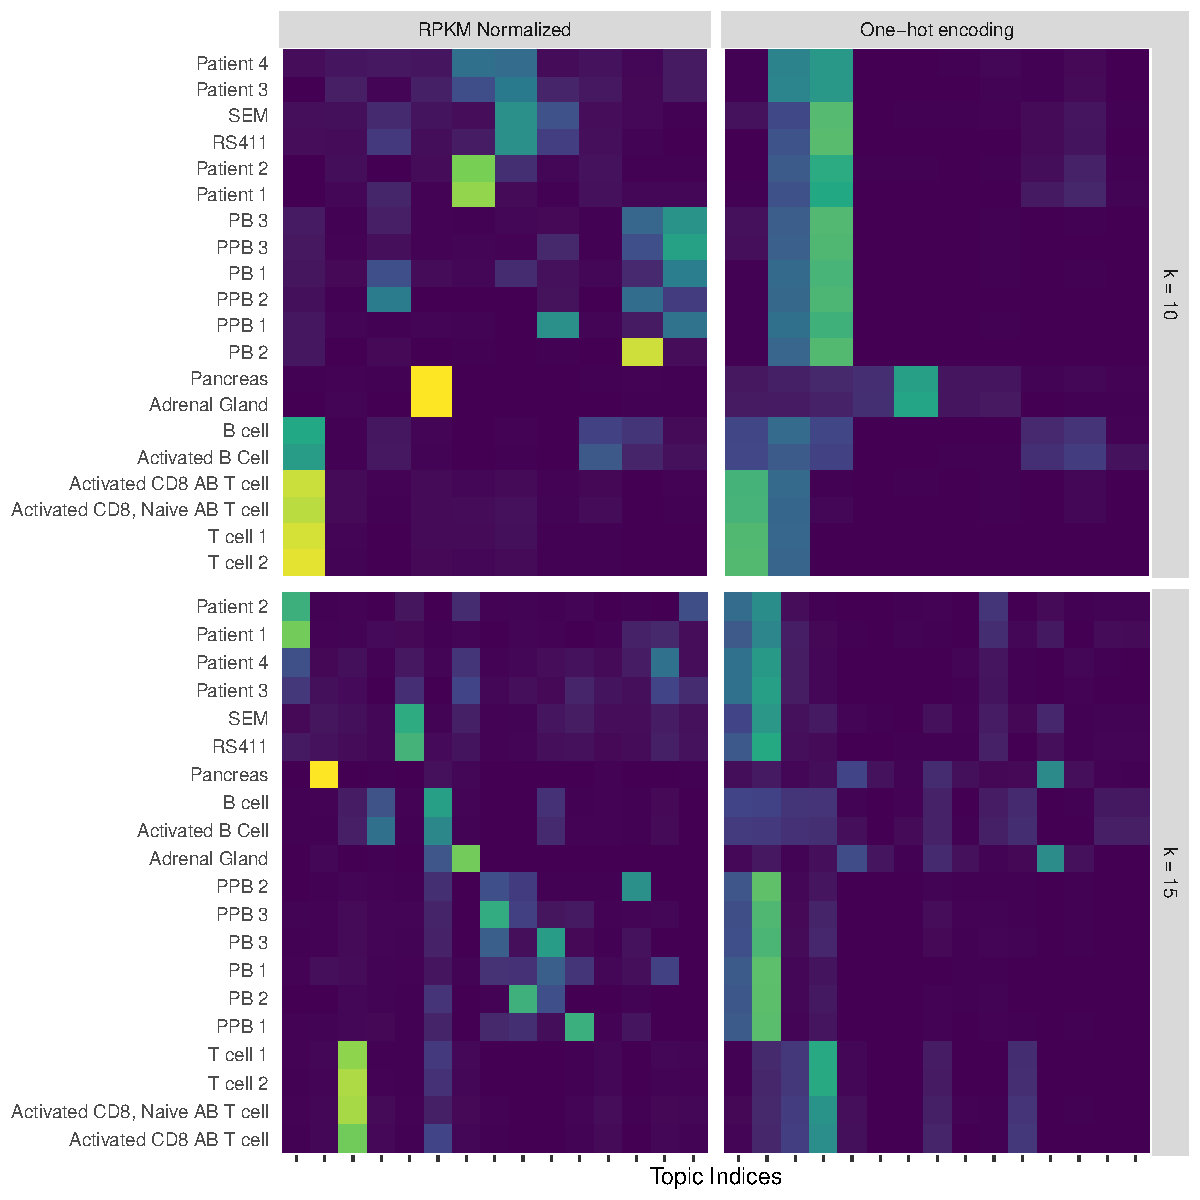
\includegraphics[width=\textwidth]{plot/ch5/encode_zoom.pdf} 
    \caption{Zoomed in plot looking at only the most related cell types to the MLL-AF4 and BCP in the ENCODE blood cell collection for $k=10$ and $k=15$ using both one-hot encoding and RPKM normalization.}
    \label{fig:encode_zoom}
\end{figure}

One of the key questions that remains to be answered is whether the unique regulatory regions identified in the previous section are still enriched in the patient topics. We took the top 100 annotated regions from topic 6 in the $k=15$ case and found that the top 100 regions in the ENCODE anlaysis included 55 of the 76 reproducible patient regions. The trend across all topics for these regions was consisent with this, most of which were predominantly involved in topic 6 (\Cref{fig:encode_pt_regions_topics}A). Of the 21 regions not within the top 100 regions for topic 6, their accessibility remained strongly associated with topic 6 (\Cref{fig:encode_pt_regions_topics}B). However, three other topics were more represented in this set, namely topics 4, 5, and 12. These topics are involvd in a variety of cell types, and interestingly Topic 4 is more active in patients 3 and 4 than in patients 1 and 2, which is the opposite of the trends previously observed. Topic 5, of which at least one of the patient-related regions has a Z-score over 30, is active in CD4 negative natural killer and T-cells, as well as K562 cancer cells. Together, threse results imply that the regulatory regions previously identified are a mix of regions uniquely active in MLL-AF4 patients and a minority which may be re-used from other cell types.  

\begin{figure}[]
    \centering
    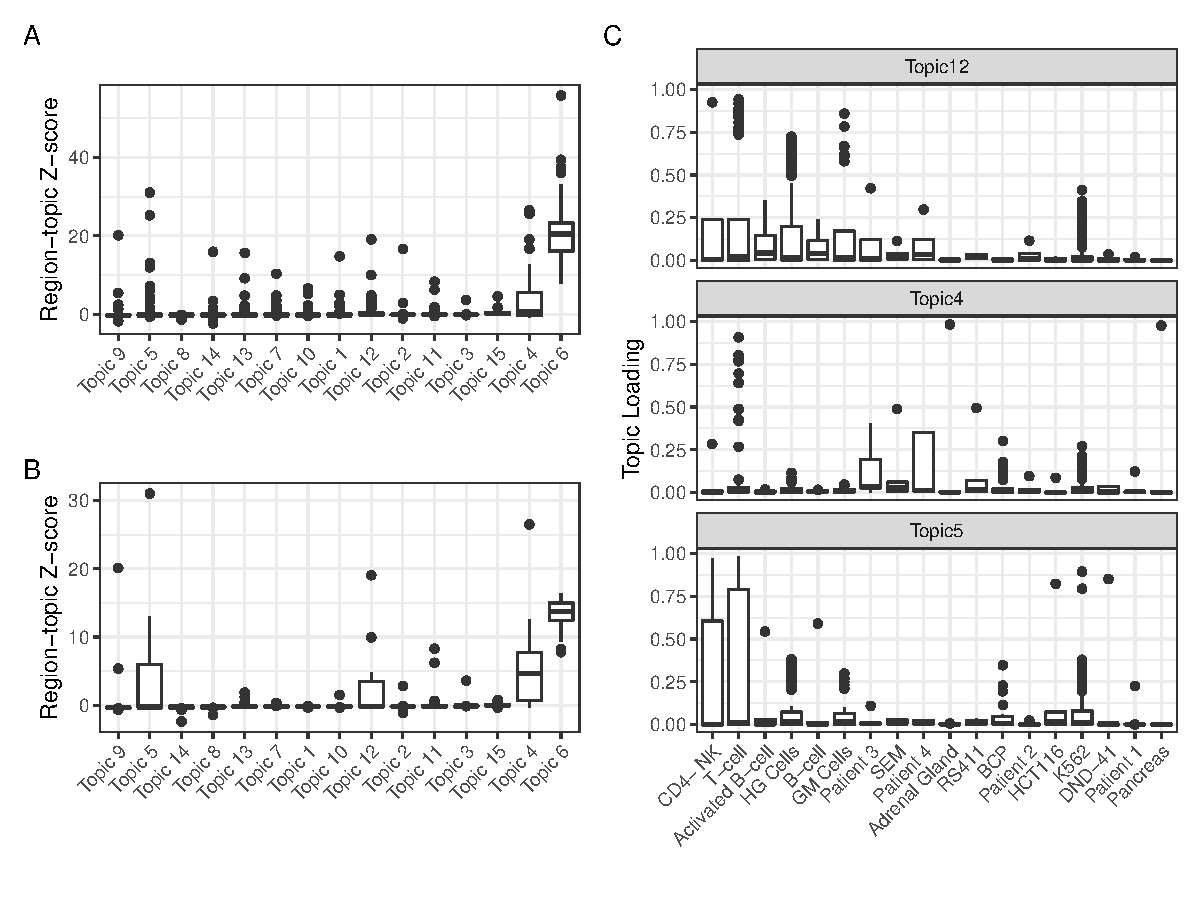
\includegraphics[width=\textwidth]{plot/ch5/encode_pt_regions.pdf} 
    \caption{Activity of 75 reproducibly identified patient-related regions within the inferred $k=15$ BLDA analysis in all of the ENCODE blood cell collection.}
    \label{fig:encode_pt_regions_topics}
\end{figure}

% For tomorrow

%- 55 of the regions from the patient topic are also found in the encode when you take out anything active in other cell types.
%- are these also the ones actually marked by things and therefore active? 

%- Correspondance between the RS411 and SEM topics just in a summary way
%- Use the ENCODE as basically a replication

%\begin{figure}
%    \centering
%    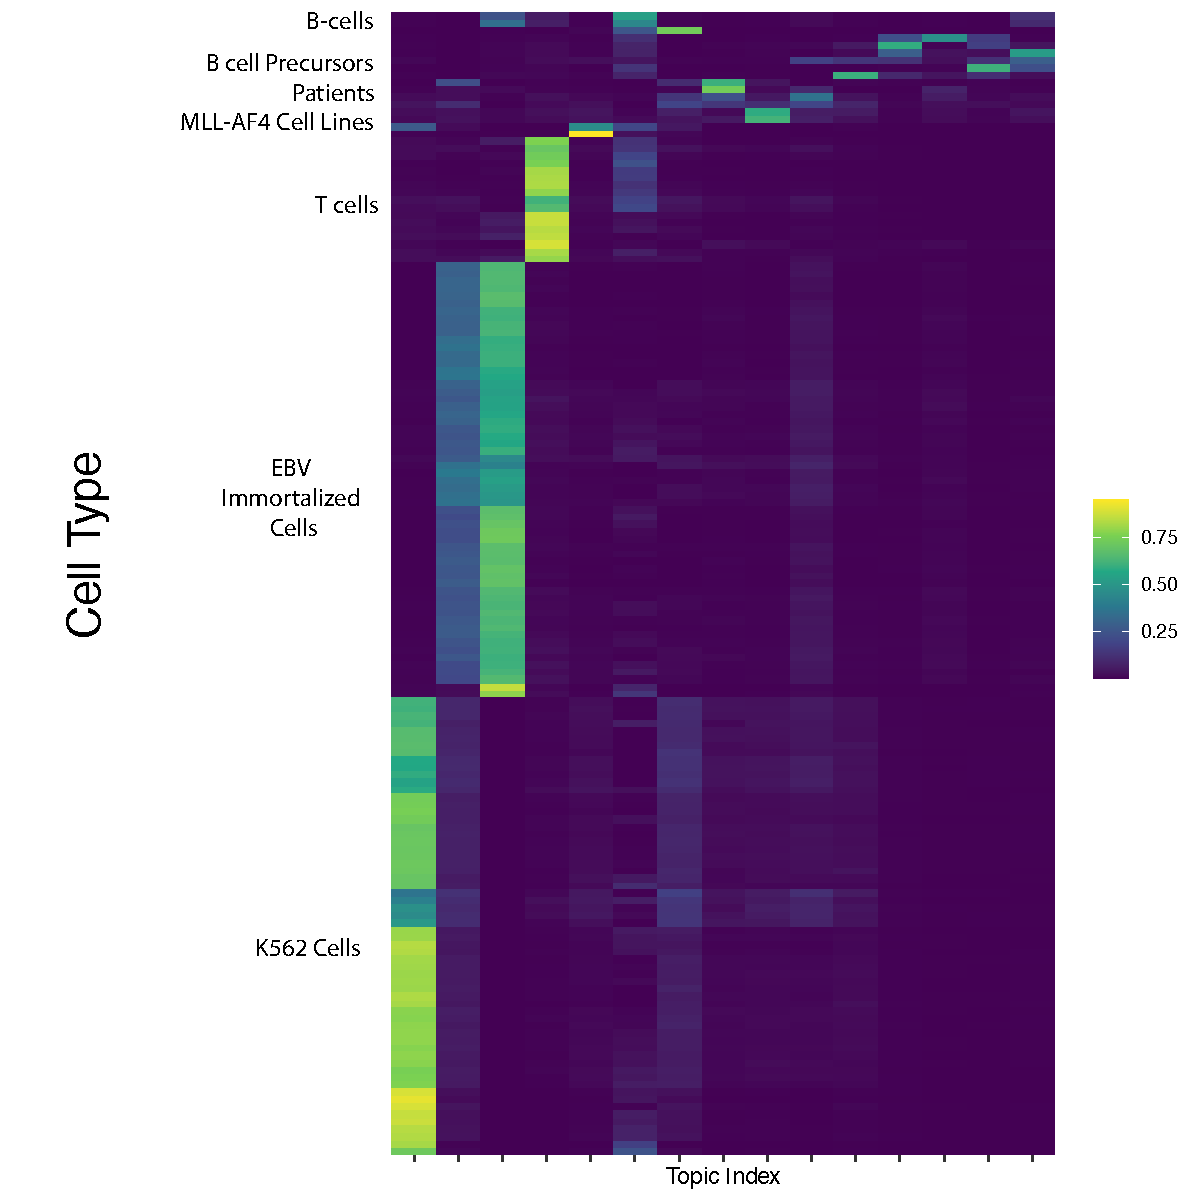
\includegraphics[width=\textwidth]{plot/ch5/mll_encode_nt15 _annotated.pdf}
%\end{figure}

\section{Discussion} \label{ch5:discussion}



% - chr10:58119757-58122125 is the promoter of ZWINT which is directly implicated in AML
%     - https://www.genecards.org/cgi-bin/carddisp.pl?gene=ZWINT
% - chr7:11,870,321-11,872,428 is promoter for THSD7A and associated with AML 
%     - https://www.ebi.ac.uk/gwas/genes/THSD7A
% - chr6:161,086,377-161,238,919 is inside of plasminogen, which is associated with AML  
%     - https://journals.sagepub.com/doi/10.1177/1076029612450771
% - chr5:27437290-27439356 is just upstream of PURPL gene, involved in p53 
% - chr5:119723091-119724864 is just upstream of PRR16, known to be involved in AML
%     - https://maayanlab.cloud/Harmonizome/gene_set/acute+myeloid+leukemia/GWASdb+SNP-Phenotype+Associations
% - chr4:62138289-62139958 intragenic ADGRL3 which is upregulated in relapsed AML samples 
%     - https://www.frontiersin.org/10.3389%2Fconf.fphar.2018.63.00023/event_abstract
% - chr4:176867295-176868639 is intragenic in GPM6A, a suspected ALL oncogene
%     - https://pubmed.ncbi.nlm.nih.gov/24916915/
%     - Also a sort of close by one, is this a regulatory region for GPM6A? chr4:177823634-177824976
% - chr4:157874799-157876498 is intragenic PDGFC, known to be related to AML blasts 
%     - https://pubmed.ncbi.nlm.nih.gov/11860452/
% - chr3:97628722-97630586 is a lncRNA that has roles in aneuploidy. 
%     - https://www.nature.com/articles/s41388-020-01601-8
% - chr3:4282880-4284204 is upstream of SETMAR (aka Metnase) controls mitotic decatenation checkpoint, AML are bad in this way
%     - https://pubmed.ncbi.nlm.nih.gov/19458360/
% - chr3:190303470-190305622 is intragenic IL1RAP, involved in AML stem cell following treatment and progression
%     - https://ashpublications.org/blood/article/126/23/4266/135849/A-Role-for-IL1RAP-in-Acute-Myelogenous-Leukemia
% - chr3:106252503-106253840 is upstream of CBLB which has known mutations in AML
%     - https://www.ncbi.nlm.nih.gov/pmc/articles/PMC1924768/
%     - Also close to ALCAM whichi s important for HSC self renewal https://pubmed.ncbi.nlm.nih.gov/23280653/ and heavily implicated in AML https://www.sciencedirect.com/science/article/pii/S0006497119339163
% - chr2:133023823-133025308 just upstream of MIR663B, involved in ALL
%     - https://www.ncbi.nlm.nih.gov/pmc/articles/PMC6884921/
% - chr18:6269486-6271399 intragenic L3MBTL4 which is a tumor suppressor gene 
%     - https://pubmed.ncbi.nlm.nih.gov/22018275/
% - Two regions very close to SETBP1. SETBP1 HOXA activation, mutant attenuates RUNX and activates MYB. Major oncogene
%     - https://pubmed.ncbi.nlm.nih.gov/28447248/
% - chr14:38593423-38595438 is upstream of SSTR1, known to be in leukemia 
%     - https://pubmed.ncbi.nlm.nih.gov/10447088/

% - chr12:24531253-24532421 intragenic SOX5 genes involved in AML: 
%     - https://www.sciencedirect.com/science/article/pii/S1044579X18301391



% - Talk about the lack of H3K79me which is weird given Tom's work on a subclass of enhancers due to MLL recruiting DOT1L. These ones don't seem to, what's going on? (cite Tom's paper)
% - Also talk about how it might not be bound by MLL-AF4 but maybe just MLL? Not sure, is this even true.


% - Monotherapies are often not very useful for KMT2A-AFF1 since relapse is so liekly. Need to figure out what the actual network of genes is an disrupt it. 
% - Construct testable hypothesis and identify important differentially accessible regions in KMT2A-AFF1
% - A lot of these regions look actually bound by MLL. So they might not be part of this downstream effect but rather unidentified regulatory regions that MLL directly influences. 
%     - Does MLL bind other than having its K methyltransferase activity? Or maybe indepdenant of DOT1L? it seems like these regions are not 79me so what's up with that 


This chapter proposes the use of topic modelling to prioritise accessible regulatory regions in a poorly understood but difficult to treat subset of leukemias.  Four childhood KMT2A-AFF1 patients were studied alongside two cell models of the same leukemia . To contrast these cancerous cells and model "normal", non-cancerous, developmental biology, we include a newly identified lymphoid committed fetal-specific cell type whose transcriptional profile closely matches known infant \glspl{all}. We additionally include a transcriptionally distinct but closely related lymphoid progenitor, ProB (PB) cells, which have known analogues in adults, but are derived from fetal sources.  We show that there are distinct accessibility patterns in the four different subsets of cells, each represented by a topic which loads uniquely onto that subset. We show that these topics encode reproducibly identified accessible regions that differentiate between KMT2A-AFF1 cancerous samples and developmentally normal \gls{bcp}, even at the stringent threshold of 100 individual regions per topic. The alternative topic modelling approach tested against, the one-hot encoding input method used by cisTopic, did not demonstrate any ability to differentiate between cell models and patient samples or PB versus PPB but did broadly differentiate between the cancerous and normal cell types, indicating at least a partial role of regions which are entirely accessible or not in the accessibility program of leukemia samples (\Cref{fig:mll_all_topic}). This bears relevance to the question of differential regulatory element usage versus differential accessibility at the same regulatory element. The fact that both methods are able to distinguish between the samples means that, on a broad level, there is at least some differential regulatory element usage between fetal KMT2Ar leukemia and the fetal PPB cells. 

Interestingly, BLDA also identified topics of regulatory elements accessible in Pre-ProB cells not shared with ProB cells, helping to illuminate fetal-specific lymphopoiesis trajectories (\Cref{fig:mll_reps}, \Cref{fig:mll_region_repro}A). A large number of these regions (102 for PPB and 158 for PB) were consistently identiied across every replicate in the top 500 regions. These regions will be the focus of more mechanistic studies tryin to understand chromatin remodelling in fetal lymphopoiesis and how it differs from the same differentiation process in adults. Understanding this process in detail is crucial to the study of fetal leukemiagenesis. These results will be particularly applicable to the study of \glspl{lsc} and how they are transformed from developmentally normal cells; is it unclear whether the pathways involved in self-renewal and maintenance of LSCs may be shared with PPB cells. In this case the topic modelling approach allows for a fine-grained dissection of known pathways and their relative contributions to different cell types. However, the aim for this chapter was explicitly to examine the regulatory regions involved in patients. The remainder of the fine-grained results will be examined in depth as time allows. 

BLDA identified a topic in each replicate that was uniquely enriched in the patient samples, most strongly in patients 1 and 2. For values of $k$ larger than 10, this topic starts to split in half, with one reprenseted strongly in patients 1 and 2 as before but the second represented more strongly in patients 3 and 4 (\Cref{fig:mll_all_topic}). Values of $k$ this large, however, seem extremely unreliable in practice, and it is unlikely that regions would be consistenly prioritized after replication. This is demonstrated by the extremely dispursed nature of the topics in \gls{bcp} samples and the lack of a central topic explaining core regulatory features shared by the entire group, which we expect to see in this case. The reasons for the consistent lack of enrichment for this topic in patients 3 and 4 are difficult to explain, but may revolve around either patient heterogeneity or sample quality. The first is an area of active research, with well known results showing very little consensus between patient derived models for different KMT2A-FPs even in terms of distinct chromatin binding \cite{Lin2016}. These previous results urge caution when interpreting observations within samples deriving from a single fusion partner. The heterogeneity within the patient population with regards to chromatin accessibility and binding efficiency of the KMT2A-AFF1 fusion protein as well as important downstream chromatin remodellers like RUNX1 is not well studied. However, in the case that substantial heterogeneity exists, and if it is important for treatment efficacy and differential prognosis, topic modelling appears to be a promising approach for dissecting these differences. The alternative explaintion is differences in patient sample quality, which is difficult to describe quantatively in this case. Though the sequencing appears to have reasonable coverage under each of the peak regions, known difficulties with preparing and isolating the necessarry cells from the patients may have prevented a completely unbiased view into their accessible chromatin. The third possibility for these differences may be differential genome instability and mutational background within the patients. Though well established that KMT2Ar cancers tend to not carry with them many functional cooperating mutations, mutations in key pathwayas such as FLT3 (frequently upregulated in KMT2Ar leukemias) have been described in pediatric and adult AML leading to extremely poor prognosis \cite{CE2014,Sternberg2005,Sexauer2017}. The genetic background of these samples is unknown, and further work is necessary to understand the contribution of genetic differences to the epigenetic profile of KMT2A-AFF1 driven leukemias.

This patient heterogeneity makes differential accessibility analysis such as the one we attempted to perform very challenging. The genes identified with the edgeR analysis bear no strong relationship to known KMT2Ar pathways, though some such as RhoU and SERF1A from \Cref{tab:table:mll_edger_genes} may have suggestive links to \gls{all} \cite{Infante2013a,Z2020,Wilson2016}. The fundamental strength with the topic modelling approach is the ability to look at variation in accessibility both collectively, between the cell lines and each individual patient, as differentially. Few regions, it seems, are uniformly different in accessibility between the different categories. This is reinforced by the inferred topic loadings, which seperate well on the different categories and suggest that fundamnetally different regulatory biology underlies the cell lines versus the patients, and that substantial heterogeneity exists even within each of those sub-classes. 

The regions picked out with the topic modelling approach appear to be mostly functional in this cellular context. Many of them have been previously annotated as enhancer or promoter elements in distantly related cell types, indicating their functional potential (\Cref{table:mll_enhancer}). Additionally, the profile of histone modifications and bound transcription factors within one of the specific patients indicates a large over-abundance of MLL binding alongside RUNX1 and PAF1c even when compared with other regions enriched for H3K4me1 and H3K27ac (\Cref{table:mll_chip}, \Cref{fig:mll_enhancer_overlap}). Interestingly, these regions are not enriched for AF4 binding, indicating that they may in fact be bound by wild-type KMT2A, though to different levels than the comparable \gls{bcp}. To our knowledge, this phenomenom has not been previously observed, and raises the possibility that the KMT2A-FP may alter the binding profile of wild-type KMT2A within the genome. These regions are actually depleted for H3K79me2 marks, which is unexpected given that KMT2A typically controls the methylation of K79 through the recruitment of DOT1L. Recent work has shown that H3K79 methylation conferred by DOT1L is essential for a subset of enhancer elements to form promoter interactions in KMT2A-AFF1 leukemia, and that inhbition of DOT1L destroys these essential connections \cite{Godfrey2019}. As the only known H3K79 methyltransferase, we can be confident that the function of regions is not dependant on DOT1L recruitment, and therefore representing a completely seperate class of KMT2A-bound but DOT1L-depleted enhancer elements that have, to our knowledge, not been previously described \cite{Q2002}. Moreso, the majority of these regions of the genome are still specifically associated with the KMT2A-AFF1 patients against the backdrop of a large set of blood cells from the ENCODE project, and they remain the most accessible cell types for all but two of the regions. This is suggestive evidence that these regions may be specifically active in these patients, at least within the hematopoetic niche. Further work will investigate these regions in the context of the entire ENCODE accessibility dataset. Though the initial results do not suggest that this is the case, as the set of cell types that these regions are previously annotated in are extremely diverse, evidence for a shared or co-opted regulatory program from a distantly related cell type would be extremely exciting. 

The next steps to validate these regions and their roles in the regulatory biology of KMT2A-AFF1 will be necessarily experimental. In order to understand which, if any, genes are being regulated by these regions, Capture-C assays will need to be performed within these specific samples. Motif enrichment within these regions, and indeed within most of the annotated sets of regions, has not been particularly illuminating as to their pathways. To understand their role in a DOT1L-indepdenant regulatory program, their enhancer-promoter interactions should be assessed with and without the use of inhibitors such as EPZ-5676. Though the possibility that these regulatory regions work completely indepdenant of this key co-factor is remote, the implications for current research into therapeutic DOT1L supression make them key candidates to understand the resistance mechanisms employed by cancer cells. The other crucial and specific aspect of these enhancers is their association with PAF1c, more typically understood as an elongation factor associated with RNA polymerase 2 \cite{Oss2017,Yang2016,Hou2019,Jaehning2010}. Very recent evidence from mouse models indicates that PAF1c occupancy may be associated with super-enhancers and is crucial for maintaining the self-renewal capacity of mouse embryonic stem-cells \cite{Ding2021}. Additionally, it is known that PAF1c is involved in the regulation of key genes involved in \gls{aml} such as HOXA9 and MEIS1, so its coordinated activity across these enhancers is of interest to the central regulatory axis of leukemia. 

In summary, this chapter has adopted a topic modelling approach that we previously developed to model chromatin accessibility patterns in KMT2A-AFF1 patients when compared to healthy fetal-specific lymphoid precursors. We identified a subset of regions bound by wildtype KMT2A but not involving DOT1L recruitment. These regions were uniquely accessible in these patients against the background of the hematopoetic niche, but there is evidence that a subset function as enhancers and promoters in distantly related cell types. Further work will focus on characterising the interactions of these regions with genes and ways in which their leukemia-specific functions may be interupted. These regulatory elements represent key targets for investigation in the search for therapeutic targets to a deadly and impactful disease.  


\section{Methods (Work in Progress)} \label{ch5:methods}

% Things to write about 

% ATAC-seq for the cell lines, patients, and BCP cells 

\subsection{Data Acquisition }

\paragraph{Patient data}

\todo{I don't have any details on these. I see in Joe's paper that one was from }

???

\paragraph{Cell Lines}

\todo{I've just copy pasted dthis from Joe's paper. Is it right?}

Two cell lines were used in this analysis. SEM cells, a KMT2A-AFF1 B cell \gls{all} cell line were purchased from DSMZ (\url{https://www.dsmz.de}). SEM cells were cul- tured in Iscove’s modified Dulbecco’s medium (IMDM) with 10\% fetal bovine serum (FBS) and 1x GlutaMAX, with cell density maintained between 5× 105/mL and 2×106/mL. RS411 cells were purchased from ATCC (\url{https://www.atcc.org}) and cultured in RPMI-1640 with 10\% FBS and 1x GlutaMAX, with cell density maintained between 5×105/mL and 1.5 ×106/mL. Cells were confirmed to be free of mycoplasma.

\paragraph{Pre-ProB and ProB cells}

ATAC-seq data was downloaded from GEO (ascession number GSE122989) as coverage track in bigWig format. 

\subsection{ATAC-seq}
\subsection{RNA-seq}
\subsection{ChIP-seq}
\subsection{Peak Calling with LanceOTron}

Peak calling on coverage data for ATAC-seq was performed with LanceOTron v1.0.1 \cite{Hentges2021}. LanceOTron was installed from Pypi here \url{https://pypi.org/project/lanceotron/1.0.1/} and used with the flags \textit{-c 0.5} and \textit{--format bed} to select only regions exceeding a peak score of 0.5 and outputting the data as a bed file for further analysis. 

\subsection{Coverage Metrics}

Megadepth was used to construct coverage metrics \cite{Wilks2021}. Peak regions were used as an annotation (flag \textit{-a}) in order to only consider coverage under regions expected to be well represented.

\subsection{Topic modelling}

Count matrices were constructed from paired coverage data and LanceOTron peak calls using the BLDA python package, available at \url{https://github.com/Chris1221/blda}. For BLDA analyses, the format was given as "bigwig", while OHE matrices were constructed with the "dummy" option. Matrices were used directly for topic modelling with a modified version of cisTopic available at \url{https://github.com/Chris1221/cisTopic_bulk}. Bayesian hyperparamter optimization is described in \Cref{ch4:hyper} and more detail on the BLDA method is given \Cref{ch4:method_blda}.


% Coverage analysis with megadepth
% Constructing count matrices with BLDA and cisTopic
% MLL blacklist
% Differential accessibility with edgeR
% Gene Ontology Enrichment
% Gene enrichments 
% Topic Modelling with BLDA
% Motif enrichment with motifscan
% Bootstrapping lncRNA from refSeq
% Bootrapping enhancer and normal background for chromatin marks and TF binding
% Finding enhancer and promoter regions with ENhancerAtlas
% Visualizing coverage data with IGV
% ENCODE Blood Cell Data Set

